\documentclass[aspectratio=1610,10pt]{beamer} %Other possible values are: 169, 149, 54, 43 and 32.
  
\input{../preambles/preamble}
\input{../preambles/preambleTikz}
\input{../preambles/preambleBeamer}


%o titulo e biblioteca na pasta local headtail
\title
  {
    An inexact scaled gradient projection method with applications in risk parity portfolios
  }

\author[M. ~Lemes] % (optional, use only with lots of authors)
  {
   \textbf{Max Lemes} \\
   Universidade Federal de Goiás.
  }

 \institute[Federal University of Goiás] % (optional, but mostly needed)


\date%[Goiânia, 07 de outubro de 2021]
  % (optional, should be abbreviation of conference name)
  {
    \textcolor{mLightBrown}{\textbf{Instituto de Matemática e Estatística.}}\\
    Goiânia, September 1, 2022.
  }
\addbibresource{presentation.bib}

\hypersetup{pdfpagemode=FullScreen}

%-----------------------------------------------------------------
\begin{document}
%-----------------------------------------------------------------

\maketitle

%         Outline      -------------------------------------------
\begin{frame}
  \frametitle{Outline}
  \tableofcontents
  % You might wish to add the option [pausesections]
\end{frame}
%-----------------------------------------------------------------



\chapter{Preliminaries}  \label{chap:Prel}
\thispagestyle{empty}

%%%%%%%%%%%%%%%%%%%%%%%%%%%%%%%%%%%%%%%%%%%%%%%%%%%%%%%%%%

In this chapter, we introduce  some notation and results used throughout our presentation.

First, we  consider the  index set  ${\mathbb{N}}:=\{0,1,2,\ldots\}$,  the usual inner  product  $\langle \cdot,\cdot \rangle$ in $\mathbb{R}^n$, and the associated Euclidean norm    $\|\cdot\|$.
Let  $f:\mathbb{R}^n \to \mathbb{R}$ be a differentiable function and $C \subseteq \mathbb{R}^n$. The  gradient $\nabla f$ of $f$ is said to be {\it Lipschitz continuous} in $C$ with constant $L>0$ if
$$
	\|\nabla f(x)-\nabla f(y)\|\leq L \|x-y\|,
$$
for all~$x, y\in C$. Combining this definition with the Fundamental Theorem of Calculus, we obtain the following result whose proof may be found in \cite[Proposition A.24]{Bertsekas1999}.

\begin{lemma} \label{Le:derivlipsch}
	Let $f:\mathbb{R}^n \to \mathbb{R}$ be a differentiable function and $C \subseteq \mathbb{R}^n$. Assume that $\nabla f$  is Lipschitz continuous in C with constant $L>0$. Then,
	\[
		f(y) - f(x) - \langle \nabla f(x), y-x \rangle \leq (L/2)\|x-y\|^2,
	\]
	for all~ $x, y\in C$.
\end{lemma}
%Let $f:\mathbb{R}^n \to \mathbb{R}$ be a differentiable function and $C \subseteq \mathbb{R}^n$ be a convex set. The function $f$ is convex on $C$, if $f(y) \geq  f(x) + \langle \nabla f(x), y-x \rangle$, for all $x, y\in C$.
Assume that $C$ is a convex set. The function $f$ is said to be \textit{convex} on $C$, if
\[
	f(y) \geq  f(x) + \langle \nabla f(x), y-x \rangle,
\]
for all $x, y\in C$. We recall  that a point ${\bar{x}} \in C$ is a {\it stationary point} for problem \eqref{eq:OptP} if
\begin{equation} \label{eq:StatPoint}
	\langle \nabla f({\bar{x}}),  x-{\bar{x}}\rangle \geq 0, \qquad \forall ~ x\in  C.
\end{equation}
Consequently, if $f$ is a convex funct{}ion  on $C$, then  \eqref{eq:StatPoint} implies that  $\bar{x} \in \Omega^*$.  We will now present some useful concepts  for the analysis of the sequence generated by the scaled  gradient method, for more details, see \cite{CombettesVu2013}.    For that,  let  $D$ be a $n\times n$ positive definite matrix and $\| \cdot \|_{D} : \mathbb{R}^{n}\rightarrow \mathbb{R}$ be  the norm  defined by
\begin{equation} \label{def:normaD}
	\|d\|_{D}:=\sqrt{\left\langle D d,d\right\rangle},\quad \forall d\in \mathbb{R}^{n}.
\end{equation}
For a fixed  constant $\mu \geq 1$,  {\it denote by  ${\cal D}_{\mu}$  the set of symmetric positive definite matrices $n\times n$ with all eigenvalues contained in the interval $[\frac{1}{\mu}, \mu]$}.  The set ${\cal D}_{\mu}$   is compact. Moreover,  for each $D\in {\cal D}_{\mu}$, it follows that $D^{-1}$ also belongs to $ {\cal D}_{\mu}$. Furthermore,  due to $D\in {\cal D}_{\mu}$,  by \eqref{def:normaD}, we obtain
\begin{equation} \label{eq:pnv}
	\frac{1}{\mu}\|d\|^2\leq \|d\|^2_{D}\leq \mu \|d\|^2, \qquad \forall d\in \mathbb{R}^n.
\end{equation}

Let us recall the the concept of  sequence  quasi-Fej\'er  monotone to a set, introduced in  \cite{CombettesVu2013}.
\begin{definition} \label{def:QuasiFejer}
	Let $(y^k)_{k\in\mathbb{N}}$ be a sequence in $\mathbb{R}^n$ and   $(D_k)_{k\in\mathbb{N}}$ be  a sequence in ${\cal D}_{\mu}$.  The sequence $(y^k)_{k\in\mathbb{N}}$ is said to be quasi-Fej\'er  monotone to a set $W\subset \mathbb{R}^n$ with respect to  $(D_k)_{k\in\mathbb{N}}$ if, there exists  a sequence $(\eta_k)_{k\in\mathbb{N}}\subset [0, +\infty)$ such that $\sum_{k\in \mathbb{N}}\eta_k<\infty$ and for  all $w\in W$, there exists a sequence $(\epsilon_k)_{k\in\mathbb{N}}\subset[0, +\infty)$ such that  $\sum_{k\in \mathbb{N}}\epsilon_k<\infty$, and
	\[
		\|y_{k+1}-w\|_{D_{k+1}}^2\leq (1+\eta_k) \|y^k-w\|_{D_k}^2+\epsilon_k,
	\]
	for    all $k\in \mathbb{N}$.
\end{definition}

The following lemma is useful to study the  quasi-Fej\'er  monotone sequence, its prove may be found in \cite[Lemma 2.2.2]{PolyakLivro1987}.
\begin{lemma} \label{le:pl}
	Let $(\alpha_k)_{k\in\mathbb{N}}$, $(\eta_k)_{k\in\mathbb{N}}$ and $(\epsilon_k)_{k\in\mathbb{N}}$ be a sequences in $[0, +\infty)$  such that $\sum_{k\in \mathbb{N}}\eta_k<\infty$ and $\sum_{k\in \mathbb{N}}\epsilon_k<\infty$. Assume that $\alpha_{k+1}\leq (1 +\eta_k)\alpha_k+\epsilon_k$, for all $k\in {\mathbb N}$. Then, $(\alpha_k)_{k\in\mathbb{N}}$ converges.
\end{lemma}

The main property of  quasi-Fej\'er  monotone sequences is stated in the following. Its proof may be found in \cite[Proposition~3.2 and Theorem 3.3]{CombettesVu2013}. For sake of completeness, we include it here.

\begin{theorem}\label{teo.qf}
	Let $(y^k)_{k\in\mathbb{N}}$ be a sequence in $\mathbb{R}^n$ and   $(D_k)_{k\in\mathbb{N}}$ be  a sequence in ${\cal D}_{\mu}$ such that $\lim_{k\rightarrow\infty}D_k={\bar D}$.   If $(y^k)_{k\in\mathbb{N}}$ is quasi-Fej\'er  monotone to a nonempty set $W\subset  \mathbb{R}^n$ with respect to $(D_k)_{k\in\mathbb{N}}$ then,  for each  $w\in W$,    the sequence  $(\|y^{k}-w\|_{D_{k}})_{k\in\mathbb{N}}$ converges. Furthermore, $(y^k)_{k\in\mathbb{N}}$ is bounded and, if each  cluster point of $(y^k)_{k\in\mathbb{N}}$ belongs to $W$, then there exists ${\bar y}\in W$ such that $\lim_{k\rightarrow\infty}y^k={\bar y}$.
\end{theorem}

\begin{proof}
	Take $w\in W$ and define the sequence $(\alpha_k)_{k\in\mathbb{N}}$, where $\alpha_k:=\|y^{k}-w\|_{D_{k}}$. Since $(y^k)_{k\in\mathbb{N}}$ is quasi-Fej\'er  monotone to $W$, Lemma~\ref{le:pl} implies that $(\alpha_k)_{k\in\mathbb{N}}$ converges. Now, by using  the  first  inequality in \eqref{eq:pnv}, we have  $\|y^{k}-w\|\leq \sqrt{\mu} \alpha_k$, for all $k\in  \mathbb{N}$.  Thus, $(y^k)_{k\in\mathbb{N}}$ is bounded. To prove the last statement, assume that   ${\bar y}, {\hat y} \in  W$   are  cluster points of $(y^k)_{k\in\mathbb{N}}$, and set   $(y^{k_i})_{i\in\mathbb{N}}$ and  $(y^{k_j})_{j\in\mathbb{N}}$  subsequences  of $(y^k)_{k\in\mathbb{N}}$ such that $\lim_{j\to +\infty} y^{k_i} = {\bar y}$ and $\lim_{j\to +\infty} y^{k_j} = {\hat y}$. It follows from the first statement that  $(\|y^{k}- {\bar y}\|_{D_{k}})_{k\in\mathbb{N}}$ and  $(\|y^{k}- {\hat y}\|_{D_{k}})_{k\in\mathbb{N}}$ are convergent. Since $\lim_{k\rightarrow\infty}D_k={\bar D}$, we have  $\lim_{k\rightarrow\infty}\|{\bar y}\|_{D_k}={\|\bar y}\|_{{\bar D}}$ and $\lim_{k\rightarrow\infty}\|{\hat y}\|_{D_k}={\|\hat y}\|_{{\bar D}}$. Hence,  due~to
	$$
		\langle y^k,  D_k({\bar y}- {\hat y})\rangle=\frac{1}{2}(\|y^{k}- {\hat y}\|_{D_{k}}^2-\|y^{k}- {\bar y}\|_{D_{k}} +\| {\bar y}\|_{D_{k}}-\| {\hat y}\|_{D_{k}}),
	$$
	for all $k\in {\mathbb N},$ we conclude that the sequence  $(\langle  y^k,  D_k({\bar y}- {\hat y})\rangle)_{k\in\mathbb{N}}$ converges.  Thus, taking into account that   $\lim_{j\to +\infty} y^{k_i} = {\bar y}$, $\lim_{j\to +\infty} y^{k_j} = {\hat y}$ and  $\lim_{k\rightarrow\infty}D_k={\bar D}$ we obtain that
	$$
		\langle  {\bar y},  {\bar D}({\bar y}- {\hat y})\rangle=\lim_{i\rightarrow\infty} \langle y^{k_i},  D_{k_i}({\bar y}- {\hat y})\rangle=\lim_{j\rightarrow\infty} \langle y^{k_j},  D_{k_j}({\bar y}- {\hat y})\rangle= \langle  {\hat y},  {\bar D}({\bar y}- {\hat y})\rangle.
	$$
	Hence, using \eqref{eq:pnv}, we obtain
	$$
		\frac{1}{\mu}\|{\bar y}- {\hat y}\|^2\leq  \|{\bar y}- {\hat y}\|^2_{\bar D}=  \langle  {\bar y},  {\bar D}({\bar y}- {\hat y})\rangle-  \langle  {\hat y},  {\bar D}({\bar y}- {\hat y})\rangle=0,
	$$
	which implies that ${\bar y}= {\hat y}$. Therefore, due to  $(y^k)_{k\in\mathbb{N}}$ be bounded, we conclude that    $(y^k)_{k\in\mathbb{N}}$ converges to ${\bar y}$.
\end{proof}


\section{Exact Projection}

\begin{frame}[t]\frametitle{Exact Projection}

  \begin{definition}[2.1]
    The \textcolor{purple}{exact  projection} of the point $v\in \mathbb{R}^{n}$ onto $C$ with respect to the norm $\| \cdot \| _{D}$, denoted by  ${\cal P}_{C}^{D}(v)$, is  defined~by
    \begin{equation*}
      {\cal P}_{C}^{D}(v):=\arg \min _{z\in C}\|z-v\|^2_{D}.
    \end{equation*}
  \end{definition}

  \bigskip
  \bigskip
  \bigskip

  \begin{lemma}[2.2]
    Let $v, w \in {\mathbb R}^n$.  Then,  $w={\cal P}_{C}^{D}(v)$ if and only if  $w\in C$ and
    \[
      \left\langle D(v-w), y-w\right\rangle \leq  0,
    \]
    for all $y \in C.$
  \end{lemma}
\end{frame}

\begin{frame}[t]\frametitle{Exact Projection}\bigskip
  \begin{figure}[!ht]
    \centering
    \includegraphics{../figures/exactProj.pdf}
    \caption{Exact projection of the point $v$ onto $C$.}
    \label{fig:exactProj}
  \end{figure}
\end{frame}

\section{Inexact Projections}


\begin{frame}
  \frametitle{Inexact Projections}

  \begin{definition}[2.5\footfullcite{BirginMartinezRaydan2003}]
    The feasible inexact projection mapping, with respect to the norm $\| \cdot \|_{D}$,   onto $C$  relative to a point  $u \in C$ and forcing parameter $\zeta\in (0, 1]$, denoted by ${\cal P}_{C,\zeta}^{D}(u,  \cdot): {\mathbb R}^n \rightrightarrows C$,  is the set-valued mapping defined as follows
    \begin{equation*}
      {\cal P}_{C,\zeta}^{D}(u, v) := \left\{w\in C:~ \|w-v\|_{D}^2\leq \zeta \| {\cal P}_{C}^{D}(v)-v\|_{D}^2+(1-\zeta)\|u-v\|_{D}^2 \right\}.
    \end{equation*}
    Each point $w\in {\cal P}_{C,\zeta}^{D}(u, v) $ is called a  \textcolor{purple}{feasible inexact projection},  with respect to the norm $\| \cdot \|_{D}$,  of $v$ onto $C$ relative to $u$ and forcing parameter $\zeta\in (0, 1]$.
  \end{definition}
\end{frame}

\begin{frame}[t]\frametitle{Inexact Projections}\bigskip
  \begin{figure}[H]
    \centering
    \includegraphics[height=0.725\textheight]{../figures/martinezProj.pdf}
    \caption{Feasible inexact projection of the point $v$ onto $C$.}
    \label{fig:martinezProj}
  \end{figure}
\end{frame}


\begin{frame}[t]\frametitle{Inexact Projections}
  \begin{definition}[2.10\footfullcite{SalzoVilla2012}\footfullcite{OrizonFabianaGilson2018}]
    The feasible inexact projection mapping, with respect to the norm $\| \cdot \|_{D}$,  onto $C$ relative to $u \in C$ and forcing parameter $\gamma\geq 0$, denoted by ${\cal R}_{C,\gamma}^{D}(u, \cdot): {\mathbb R}^n \rightrightarrows C$,  is the set-valued mapping defined as follows
    \begin{equation*}
      {\cal R}_{C,\gamma}^{D}(u, v):= \left\{w\in C:~\left\langle D(v-w), y-w \right\rangle \leq \gamma \|w-u\|_{D}^2, \quad \forall~ y \in C \right\}.
    \end{equation*}
    Each point $w\in {\cal R}_{C,\gamma}^{D}(u, v)$ is called a \textcolor{purple}{feasible inexact projection},  with respect to the norm $\| \cdot \|_{D}$,  of $v$ onto $C$ relative to $u$ and forcing parameter $\gamma\geq 0$.
  \end{definition}
\end{frame}


\begin{frame}[t]\frametitle{Inexact Projections}
  Let $u\in C$, $v\in \mathbb{R}^n$, $w\in{\cal R}_{C,\gamma}^{D}(u, v)$ be as stated in Definition 2.10, $0\leq t <1$ and
  $$
    w_t = w+t(v-w).
  $$
  Since
  $$
    \left\langle D(v-w), y-w \right\rangle \leq \gamma \|w-u\|_{D}^2,
  $$
  for all $y\in C$ we have
  \begin{align*}
    \begin{aligned}
      \left\langle D(v-w_t), y-w_t \right\rangle & \leq  (1-t)\left[ \gamma \|w-u\|_D^2 - t\|v-w\|_D^2 \right].
    \end{aligned}
  \end{align*}

  It follows that, for all
  \begin{equation}
    t \geq \frac{\gamma \|w-u\|_D^2}{\|v-w\|_D^2}
  \end{equation}
  $w_t$ satisfies
  \begin{equation}
    \left\langle D(v-w_t), y-w_t \right\rangle\leq 0.
  \end{equation}
\end{frame}


% \begin{frame}[t]\frametitle{Inexact Projections}\bigskip   
%   \begin{figure}[H]
%   %\begin{adjustwidth}{2.2cm}{2.2cm}
%   \begin{subfigmatrix}{2}
%     \subfigure[Geometric interpretation.]{\includegraphics{../figures/condProj1.pdf}}
%     \subfigure[Example of ${\cal R}_{C,\gamma}^{D}(u, v)$.]{\includegraphics{../figures/condProj2.pdf}}
%   \end{subfigmatrix}
%   \caption{Geometric interpretation of projection ${\cal R}_{C,\gamma}^{D}(u, v)$.}
%   \label{fig:condProj1}
%   %\end{adjustwidth}
% \end{figure}
% \end{frame}

% \begin{frame}[t]\frametitle{Inexact Projections}\bigskip   
% \begin{figure}[H]
%   %\begin{adjustwidth}{2.2cm}{2.2cm}
%   \begin{subfigmatrix}{3}
%     \subfigure[]{\includegraphics{../figures/condProj3.pdf}}
%     \subfigure[]{\includegraphics{../figures/condProj4.pdf}}
%     \subfigure[]{\includegraphics{../figures/condProj5.pdf}}
%   \end{subfigmatrix}
%   \caption{Examples of regions given by inexact projection ${\cal R}_{C,\gamma}^{D}(u, v)$.}
%   \label{fig:baseline}
%   %\end{adjustwidth}
% \end{figure}
% \end{frame}

% \begin{frame}[t]\frametitle{Inexact Projections}\bigskip   
% \begin{figure}[H]
%   \begin{subfigmatrix}{3}
%     \subfigure[]{\includegraphics[width=0.3\textwidth]{../figures/condProj6.pdf}}
%     \subfigure[]{\includegraphics[width=0.3\textwidth]{../figures/condProj7.pdf}}
%     \subfigure[]{\includegraphics[width=0.37\textwidth]{../figures/condProj8.pdf}}
%   \end{subfigmatrix}
%   \caption{Examples of regions given by inexact projection ${\cal R}_{C,\gamma}^{D}(u, v)$.}
%   \label{fig:baseline}
% \end{figure}
% \end{frame}


\begin{frame}[t]\frametitle{Inexact Projections}
  \begin{lemma}[2.14]
    Let $v \in {\mathbb R}^n$, $u \in C$, $\gamma \geq 0$  and $\zeta\in (0, 1]$.  If  $0 \leq \gamma <1/2$ and $\zeta=1-2\gamma$, then
    \[
      {\cal R}_{C,\gamma}^{D}(u, v) \subset {\cal P}_{C,\zeta}^{D}(u, v).
    \]
  \end{lemma}

  \bigskip
  \bigskip
  \bigskip

  \begin{proposition}[2.17]
    Let $v \in {\mathbb R}^n$, $u \in C$ and assume that $C$ is a \textcolor{purple}{bounded set}. Then, for each $0<\gamma < 1/2$,     there exist $0 < \zeta  <1$ such that
    \[
      {\cal P}_{C,\zeta}^{D}(u, v)  \subseteq    {\cal R}_{C,\gamma}^{D}(u, v)
    \]
  \end{proposition}
\end{frame}


\begin{frame}[t]\frametitle{Inexact Projections}
  \begin{lemma}[2.18]
    Let $x \in C$, $\alpha > 0$ and  $z(\alpha) = x-\alpha D^{-1} \nabla f(x)$. Take $w(\alpha) \in  {\cal P}_{C,\zeta}^{D}(x, z(\alpha))$ with $\zeta\in (0, 1]$. Then, there hold
    \begin{enumerate}[(i)]
      \item {\small $\displaystyle \langle \nabla f(x), w(\alpha) - x\rangle \leq -\frac{1}{2\alpha} \|w(\alpha) -x\|_{D}^2 +   \frac{\zeta}{2\alpha} \left[\| {\cal P}_{C}^{D}(z(\alpha))-z(\alpha)\|_{D}^2 - \|x-z(\alpha)\|_{D}^2\right]$;}

      \item the point $x$ is stationary for problem \eqref{eq:OptP} if, and only if, $x \in {\cal P}_{C,\zeta}^{D}(x, z(\alpha))$;

      \item if  $x \in C$ is a nonstationary point for problem \eqref{eq:OptP}, then $\Big\langle \nabla f(x), w(\alpha) - x \Big\rangle < 0$. Equivalently, if there exists ${\bar \alpha}>0$ such that $\Big\langle \nabla f(x), w({\bar \alpha}) - x \Big\rangle \geq 0$, then $x$ is stationary for problem \eqref{eq:OptP}.
    \end{enumerate}
  \end{lemma}
\end{frame}
\chapter{Inexact scaled gradient method} \label{chap:SGM}
\thispagestyle{empty}


The aim of this chapter is to present an  inexact  version of SGP method, which   inexactness are in two distinct senses.  First,  we  use  a version of the inexactness scheme introduced in \cite{BirginMartinezRaydan2003},  and also a variation of the one appeared in \cite{VillaSalzo2013},  to compute an inexact projection  onto the feasible  set   allowing an appropriate  relative error tolerance. Second,  using the  inexactness  conceptual scheme for  nonmonotones    line  search   introduced  in  \cite{GrapigliaSachs2017, SachsSachs2011}, a step size is computed  to define the next iterate.  The statement of the  conceptual algorithm is as follows.

\begin{algorithm}[H]\small%\footnotesize
	\addtocontents{loa}{\def\string\figurename{Algorithm}}
	%\begin{algorithmic}[h]
	\begin{description}
		\item[Step 0.] Choose  $\sigma,{\zeta_{\min}}  \in (0, 1)$, $\delta_{\min}\in [0, 1)$, $0<\underline \omega<\bar \omega<1$, $0 < \alpha_{\min} \leq \alpha_{\max}$ and $\mu \geq1$. Let $x^0\in C$, $\nu_0\geq 0$ and set $k \gets 0$.
		\item[Step 1.] Choose positive real numbers $\alpha_k$ and $\zeta_k$, and a positive definite matrix $D_k$ such that
			\begin{equation} \label{eq:TolArm}
				\alpha_{\min}\leq \alpha_k \leq \alpha_{\max}, \qquad \qquad 0 <{\zeta_{\min}}<\zeta_k \leq 1, \qquad \qquad D_k\in {\cal D}_{\mu}.
			\end{equation}
			Compute $w^{k}\in C$  as any feasible inexact projection  with respect to the norm $\| \cdot \| _{D_k}$ of $z^k := x^{k}-\alpha_k D_k^{-1}\nabla f(x^{k})$ onto $C$ relative to $x^{k}$  with forcing parameter $\zeta_k$, i.e.,
			\begin{equation} \label{eq:PInexArm}
				w^k \in   {\cal P}_{C, \zeta_k}^{D_k}(x^{k}, z^k).
			\end{equation}
			If $w^k= x^k$, then {\bf stop} declaring convergence.
		\item[Step 2.]  Set $\tau_{\textrm{trial}} \gets 1$. If
			\begin{equation}\label{eq:TkArm}
				f\big(x^{k}+ \tau_{\textrm{trial}}(w^k - x^{k})\big) \leq f(x^{k}) + \sigma \tau_{\textrm{trial}}\big\langle \nabla f(x^{k}), w^k - x^{k} \big\rangle + \nu_k,
			\end{equation}
			then  $\tau_k\gets \tau_{\textrm{trial}}$, define the next iterate $x^{k+1}$ as
			\begin{equation} \label{eq:IterArm}
				x^{k+1} = x^{k} + \tau_k (w^k - x^{k}),
			\end{equation}
			and go to {\bf Step 3}. Otherwise, choose $\tau_{\textrm{new}} \in [\underline\omega \tau_{\textrm{trial}}, \bar\omega \tau_{\textrm{trial}} ]$, set $\tau_{\textrm{trial}} \gets \tau_{\textrm{new}}$, and repeat test \eqref{eq:TkArm}.

		\item[Step 3.]  Take  $\delta_{k+1}\in [\delta_{\min}, 1]$ and choose    $\nu_{k+1}\in {\mathbb R}$ satisfying
			\begin{equation} \label{eq:nuk}
				0\leq \nu_{k+1}\leq (1-\delta_{k+1})\big[f(x^{k})+\nu_{k}-f(x^{k+1})\big].
			\end{equation}
			Set $k\gets k+1$ and go to \textbf{Step~1}.
	\end{description}
	%	\end{algorithmic}

	\caption{SGP with inexact projection and nonmonotone line search}
	\label{Alg:GeneralSeach}
\end{algorithm}

\bigskip

Let us describe the main features of Algorithm~\ref{Alg:GeneralSeach}. In Step~1,  we first  choose   $\alpha_{\min}\leq \alpha_k \leq \alpha_{\max}$, $0 < \zeta_{\min} \leq \zeta_k  < 1$, and  $D_k\in  {\cal D}_{\mu}$. Then, by using some (inner) procedure, such as those specified in Chapter~\ref{chap:SubInexProj}, we compute $w^k$ as any feasible inexact projection of $z^k = x_k - \alpha_kD_k^{-1}\nabla f(x_k)$ onto the feasible set $C$ relative to the previous iterate $x^k$ with forcing parameter $\zeta_k$. If $w^k= x^k$, then Lemma~\ref{Le:ProjProperty}{\it (ii)} implies that $x^{k}$ is a solution of  problem \eqref{eq:OptP}.  Otherwise,  $w^k\neq  x^k$ and Lemma~\ref{Le:ProjProperty}{\it (i)}  implies  that $ w^k- x^k$ is a descent direction of $f$ at $x^k$, i.e.,  $\langle \nabla f(x^k), w^k- x^k \rangle < 0$.    Hence, in Step~2, we employ a nonmonotone line search  with tolerance parameter $\nu_k\geq 0$ to compute a step size  $\tau_k \in (0, 1]$,  and  the next iterate is computed as in \eqref{eq:IterArm}. Finally, due to  \eqref{eq:TkArm} and  $\delta_{k+1}\in [\delta_{\min}, 1]$, we have $$0\leq (1-\delta_{k+1})\big[f(x^{k})+\nu_{k}-  f(x^{k+1})\big].$$  Therefore, the next   tolerance parameter $\nu_{k+1}\in {\mathbb R}$ may be chosen satisfying \eqref{eq:nuk}  in Step~3, completing the iteration.

It is worth mentioning that the conditions in \eqref{eq:TolArm}  allow combining several strategies for choosing the step sizes $\alpha_k$  and the matrices $D_k$  to accelerate the performance of the classical gradient method.   Strategies  of choosing the step sizes $\alpha_k$  and the matrices $D_k$ have their origin in the study of the gradient  method  for unconstrained  optimization,  papers dealing with this issue include  but are not limited to \cite{BB1988, DaiHage2006, Serafino2018, Friedlander1999, Dai2006}, see also  \cite{BonettiniPrato2015, DaiFletcher2005, DaiFletcher2006, Polyak_Levitin1966}. More details  about   selecting  step sizes $\alpha_k$  and matrices $D_k$  may be found in the recent  review  \cite{bonettini2019recent} and  references therein.


Below, we present some  particular instances  of the parameter   $\delta_k\geq 0$ and  the non-monotonicity tolerance parameter $ \nu_ {k} \geq 0$  in Step~3.

\begin{enumerate}
	\item {\it Armijo line search}

	      Taking  $\nu_k\equiv 0$, the line search   \eqref{eq:TkArm}  is the well-known (monotone) Armijo line search, see \cite[Section 2.3]{Bertsekas1999}. In this case, we  may take  $\delta_k\equiv 1$ in Step~3.

	\item {\it Max-type line search}

	      The earliest nonmonotone line search strategy  was proposed  in \cite{Grippo1986}. Let $M>0$ be an integer parameter. In an iteration $k$, this strategy requires a step size $\tau_k>0$ satisfying
	      \begin{equation}\label{eq:grippo}
		      f\big(x^{k}+ \tau_k(w^k - x^{k})\big) \leq \max_{0\leq j\leq m_k}f(x^{k-j}) + \sigma \tau_k\big\langle \nabla f(x^{k}), w^k - x^{k} \big\rangle,
	      \end{equation}
	      where $m_0=0$ and $0\leq m_k\leq \min\{m_{k-1}+1, M\}$.  To simplify the notations,  we define $$f(x^{\ell(k)}):=\max_{0\leq j\leq m_k}f(x^{k-j}).$$  In order to identify \eqref{eq:grippo} as a particular instance of \eqref{eq:TkArm}, we  set
	      \begin{equation} \label{eq:casg}
		      \nu_{k}= f(x^{\ell(k)})-f(x^k), \quad 0=\delta_{\min}\leq \delta_{k+1}\leq  [f(x^{\ell(k)})- f(x^{\ell(k+1)})]/[f(x^{\ell(k)})-f(x^{k+1})].
	      \end{equation}
	      Parameters $\nu_{k}$ and $\delta_{k+1}$ in \eqref{eq:casg} satisfy the corresponding conditions in Algorithm~\ref{Alg:GeneralSeach}, i.e.,  $\nu_{k} \geq 0$ and  $\delta_{k+1}\in [\delta_{\min}, 1]$ (with   $\delta_{\min}=0$)  satisfy \eqref{eq:nuk}.  In fact, the definition of $f(x^{\ell(k)})$ implies that   $ f(x^{k})\leq f(x^{\ell(k)})$ and hence $\nu_{k} \geq 0$.  Due to  $\langle \nabla f(x^{k}), w^k - x^{k} \rangle<0$,   it follows from  \eqref{eq:TkArm} that $f(x^{\ell(k)})-f(x^{k+1})>0$. Since   $m_{k+1}\leq m_{k}+1$, we conclude that  $$f(x^{\ell(k)})-f(x^{\ell(k+1)}) \geq 0.$$
	      Hence, since $ f(x^{k+1})\leq f(x^{\ell(k+1)})$, we obtain $\delta_{k+1}\in [0, 1]$.  Moreover,  \eqref{eq:nuk} is equivalent  to
	      $$
		      \delta_{k+1}[f(x^{k})+\nu_{k}-f(x^{k+1})] \leq(f(x^{k})+\nu_{k}) -  (f(x^{k+1})+ \nu_{k+1}),
	      $$
	      which in turn, taking into account  that $\nu_{k}= f(x^{\ell(k)})-f(x^k)$, is equivalent to second inequality in \eqref{eq:casg}. Thus, \eqref{eq:grippo} is a particular instance of \eqref{eq:TkArm} with  $\nu_{k}$ and $\delta_{k+1}$ defined in \eqref{eq:casg}.  Therefore,  Algorithm~\ref{Alg:GeneralSeach} has as a particular instance the  inexact   projected  version of the scaled gradient method employing   the nonmonotone line search  \eqref{eq:grippo}. This version has been considered in \cite{BirginMartinezRaydan2003}; see also  \cite{Bonettini2009, WangLiu2005}.


	\item {\it Average-type line search}

	      Let us first recall the definition of the sequence of ``cost updates' $(c_k)_{k\in\mathbb{N}}$  that  characterizes the nonmonotone line search proposed in  \cite{ZhangHager2004}. Let   $0\leq \eta_{\min}\leq \eta_{\max}<1$,   $c_0 = f(x_0)$ and  $q_0 = 1$. Choose $\eta_k\in [\eta_{\min},  \eta_{\max}]$ and set
	      \begin{equation} \label{eq:zhs}
		      q_{k+1}=\eta_kq_{k}+1, \qquad c_{k+1} = [\eta_kq_kc_k + f(x^{k+1})]/q_{k+1}, \qquad \forall k \in \mathbb{N}.
	      \end{equation}
	      Some algebraic manipulations show that the sequence defined in   \eqref{eq:zhs} is equivalent to
	      \begin{equation} \label{eq:zhsn}
		      c_{k+1} = (1-1/q_{k+1})c_{k}+f(x^{k+1})/q_{k+1}, \qquad \forall k \in \mathbb{N}.
	      \end{equation}
	      Since \eqref{eq:nuk} is equivalent  to
	      $$
		      f(x^{k+1})+ \nu_{k+1}\leq (1-\delta_{k+1})(f(x^{k})+\nu_{k})+\delta_{k+1}f(x^{k+1}),
	      $$
	      it follows from \eqref{eq:zhsn} that  letting  $\nu_{k}=c_k-f(x^k)$ and $\delta_{k+1}=1/q_{k+1}$, Algorithm~\ref{Alg:GeneralSeach} becomes the  inexact   projected  version of the scaled gradient method employing   the nonmonotone line search proposed in   \cite{ZhangHager2004}.  Finally,  considering that $q_0 = 1$ and  $\eta_{\max}<1$, the  first equality in   \eqref{eq:zhs} implies  that
	      $$
		      q_{k+1}=1+\sum_{j=0}^{k}\prod_{i=0}^{j}\eta_{k-i}\leq \sum_{j=0}^{+\infty} \eta_{\max}^{j}=1/(1-\eta_{\max}).
	      $$
	      In this case, due to $\delta_{k+1}=1/q_{k+1}$, we may take   $\delta_{\min}=1-\eta_{\max}>0$ in  Step~3.  For gradient projection methods employing   the nonmonotone Average-type line search see, for example, \cite{Paulo2007,Schuverdt2019,  Xihong2018}.
\end{enumerate}
\begin{remark}\normalfont \label{rem:outras}
	The general line search in Step~2 of Algorithm~\ref{Alg:GeneralSeach} with  parameters  $\delta_{k+1}$  and  $\nu_{k}$ properly chosen in Step~3, also contains as particular cases the nonmonotone line searches  that appeared in  \cite{Ahookhosh2012,MoLiuYan2007}, see also \cite{GrapigliaSachs2017}.
\end{remark}\normalfont
%%%%%%%%%%%%%%%%%%%%%%%%%%%%%%%%%%%%%%%%%%%%%
\section{Partial asymptotic convergence analysis} \label{Sec:PartialConvRes}
The goal  of this section is to present a partial  convergence result for  the sequence $(x^k)_{k\in\mathbb{N}}$ generated by Algorithm~\ref{Alg:GeneralSeach}, namely, we will prove that every cluster point of $(x^k)_{k\in\mathbb{N}}$ is stationary for problem~\eqref{eq:OptP}.  For that, we state a result that is contained in the proof of \cite[Theorem 4]{GrapigliaSachs2017}.
\begin{lemma} \label{le:fkvk}
	For all $k \in \mathbb{N}$,
	$$
		0\leq \delta_{k+1}\big[ f(x^{k})+\nu_{k}-  f(x^{k+1})\big] \leq \big( f(x^{k})+\nu_{k}\big) - \big( f(x^{k+1})+\nu_{k+1}\big).
	$$
	As consequence the sequence   $\left(f(x^k)+\nu_k\right)_{k\in\mathbb{N}}$ is    non-increasing.
\end{lemma}

Next, we present our first convergence result. It is worth noting that, just as in the classical projected gradient method, we do not need to assume that $f$ has a bounded sub-level  set.

\begin{proposition} \label{pr:statArm}
	Assume that $\lim_{k\to +\infty} \nu_{k} = 0$.   Then, Algorithm~\ref{Alg:GeneralSeach} stops in a finite number of iterations at a stationary point of problem \eqref{eq:OptP}, or generates an infinite sequence $(x^k)_{k\in\mathbb{N}}$ for which every cluster point is stationary for problem~\eqref{eq:OptP}.
\end{proposition}
\begin{proof}
	First, assume that $(x^k)_{k\in\mathbb{N}}$ is finite. In this case, according to Step~1,   there exists $k \in \mathbb{N}$ such that $x^k = w^k \in{\cal P}_{C, \zeta_k}^{D_k}(x^{k}, z^k)$, where $z^k = x^{k}-\alpha_k D_k^{-1}\nabla f(x^{k})$, $0 <{\bar \zeta}<\zeta_k \leq 1$ and $\alpha_k > 0$. Therefore, applying Lemma~\ref{Le:ProjProperty}{\it (ii)} with $x = x^{k}$, $\alpha = \alpha_k$ and $\zeta= \zeta_k$, we conclude that $x^k$ is stationary for problem~\eqref{eq:OptP}.  Now, assume that $(x^k)_{k\in\mathbb{N}}$ is infinite.   Let ${\bar x}$ be a cluster point of $(x^k)_{k\in\mathbb{N}}$ and $(x^{k_j})_{j\in\mathbb{N}}$ be a subsequence of $(x^k)_{k\in\mathbb{N}}$ such that $\lim_{j\to +\infty} x^{k_j} = \bar{x}$. Since $C$ is closed and  $(x^k)_{k\in\mathbb{N}}\subset C$,  we have $\bar{x} \in C$. Moreover,     since  $\lim_{k\to +\infty} \nu_{k} = 0$, we have
	$$\lim_{j\to +\infty}\left(f(x^{k_j}) +\nu_{k_j}\right) =f(\bar{x}).$$
	Hence, considering that  $\lim_{k\to +\infty} \nu_{k} = 0$ and Lemma~\ref{le:fkvk} implies  that   $\left(f(x^k)+\nu_{k}\right)_{k\in\mathbb{N}}$  is  non-increasing, we conclude that
	$$\lim_{k\to +\infty} f(x^{k})= \lim_{k\to +\infty}\left(f(x^{k}) +\nu_{k}\right) =f(\bar{x}).$$
	On the other hand,  due to  $w^k \in {\cal P}_{C, \zeta_k}^{D_k}(x^{k}, z^k)$, where $z^k = x^{k}-\alpha_k \nabla f(x^{k})$,  Definition~\ref{def:InexactM} implies
	\begin{equation} \label{eq:bsw}
		\|w^{k_j} - z^{k_j}\|_{D_k}^2\leq \zeta_{k_j} \| {\cal P}_{C}^{ D_k}(z^{k_j})-z^{k_j}\|_{D_k}^2+(1-\zeta_{k_j})\|x^{k_j}-z^{k_j}\|_{D_k}^2 .
	\end{equation}
	Considering that $(\alpha_k)_{k\in\mathbb{N}}$ and $(\zeta_k)_{k\in\mathbb{N}}$ are bounded, $(D_k)_{k\in\mathbb{N}}\subset  {\cal D}_{\mu}$,  $(x^{k_j})_{j\in\mathbb{N}}$ converges to ${\bar x}$ and $\nabla f$ is continuous, the last inequality together Remark~\ref{re:cproj} and \eqref{eq:pnv}  imply that $(w^{k_j})_{j\in\mathbb{N}}\subset C$ is also bounded. Thus, we assume without loss of generality that $\lim_{j\to +\infty} w^{k_j} = \bar{w}\in C$.  In addition,  taking into account that  $x^k \neq w^k$ for all $k = 0,1, \ldots$, applying Lemma~\ref{Le:ProjProperty}{\it (i)} with $x = x^{k}$, $\alpha = \alpha_k$, $z(\alpha)=z^k$ and $\zeta= \zeta_k$, we obtain  that $\langle \nabla f(x^k), w^k- x^k \rangle < 0$, for all $k = 0, 1, \ldots$. Therefore,  \eqref{eq:TkArm} and \eqref{eq:IterArm} imply that
	\begin{equation}\label{eq:fmotArmf}
		0 < -\sigma\tau_{k} \big\langle \nabla f(x^{k}), w^{k}-x^{k} \big\rangle \leq f(x^{k}) +\nu_k- f(x^{k+1}), \qquad \forall ~k \in \mathbb{N}.
	\end{equation}
	Now, due $\tau_k \in (0,1]$, for all $k=0,1, \ldots$, we also assume without loss of generality that $\lim_{j \to +\infty} \tau_{k_j} = \bar{\tau} \in [0,1].$
	Therefore,   since $\lim_{k\to +\infty} f(x^{k}) =f(\bar{x})$ and $\lim_{k\to +\infty} \nu_{k} = 0$, taking limit in \eqref{eq:fmotArmf} along the  subsequences  $(x^{k_j})_{j\in\mathbb{N}}$,  $(w^{k_j})_{j\in\mathbb{N}}$ and $(\tau_{k_j})_{j\in\mathbb{N}}$  yields
	$
		\bar{\tau} \big\langle \nabla f(\bar{x}), \bar{w}- \bar{x} \big\rangle=0.
	$
	We have two possibilities: $\bar{\tau} > 0$ or $\bar{\tau} = 0$. If $\bar{\tau} > 0$, then  $\big\langle \nabla f(\bar{x}), \bar{w}- \bar{x} \big\rangle = 0.$
	Now, we  assume that $\bar{\tau} = 0$. In this case, for all $j$ large enough, there exists $0<\hat\tau_{k_j}\leq \min\{1,\tau_{k_j}/\underline\omega\}$ such that
	\begin{equation}\label{eq:ffA10}
		f\big(x^{k_j}+\hat\tau_{k_j} (w^{k_j} - x^{k_j})\big) > f(x^{k_j}) + \sigma \hat\tau_{k_j} \big\langle \nabla f(x^{k_j}), w^{k_j} - x^{k_j} \big\rangle +\nu_{k_j}.
	\end{equation}
	On the other hand, by the mean value theorem, there exists $\xi_{k_j}\in(0,1)$ such that
	$$\langle \nabla f\big(x^{k_j}+\xi_{k_j}\hat\tau_{k_j} (w^{k_j} - x^{k_j})\big), \hat\tau_{k_j} (w^{k_j} - x^{k_j})\rangle = f\big(x^{k_j}+\hat\tau_{k_j} (w^{k_j} - x^{k_j})\big) - f(x^{k_j}).$$
	Combining this equality with \eqref{eq:ffA10}, and taking into account that $\nu_{k_j}\geq 0$, we have
	$$\langle \nabla f\big(x^{k_j}+\xi_{k_j}\hat\tau_{k_j} (w^{k_j} - x^{k_j})\big), \hat\tau_{k_j} (w^{k_j} - x^{k_j})\rangle>\sigma \hat\tau_{k_j} \big\langle \nabla f(x^{k_j}), w^{k_j} - x^{k_j} \big\rangle,$$
	for $j$ large enough. Since $0<\hat\tau_{k_j}\leq \min\{1,\tau_{k_j}/\underline\omega\}$, it follows that $\lim_{j\to\infty} \hat\tau_{k_j} \|w^{k_j} - x^{k_j}\|=0$. Then, dividing both sides of the above inequality by $\hat\tau_{k_j}>0$ and taking limits as $j$ goes to $+\infty$, we conclude that
	$$ \langle \nabla f(\bar{x}), \bar{w}-\bar{x} \rangle \geq \sigma \langle \nabla f(\bar{x}), \bar{w}-\bar{x} \rangle.$$
	Hence, due to $\sigma \in (0, 1)$, we obtain $\langle \nabla f(\bar{x}), \bar{w}-\bar{x} \rangle \geq 0$. We recall that $\langle \nabla f(x^{k_j}), w^{k_j}- x^{k_j} \rangle < 0$, for all $j=0, 1, \ldots$, which taking limit as $j$ goes to $+\infty$ yields $\langle \nabla f(\bar{x}), \bar{w}-\bar{x} \rangle \leq 0.$ Hence, we also have $\langle \nabla f(\bar{x}), \bar{w}-\bar{x} \rangle = 0$. Therefore, for any of the two possibilities, $\bar{\tau} > 0$ or $\bar{\tau} = 0$, we have $\langle \nabla f(\bar{x}), \bar{w}-\bar{x} \rangle = 0$. On the other hand,  since  $(\alpha_k)_{k\in\mathbb{N}}$ and    $(\zeta_k)_{k\in\mathbb{N}}$   are  bounded, we also assume without loss of generality that $\lim_{j \to +\infty} \alpha_{k_j} = \bar{\alpha} \in [\alpha_{\min}, \alpha_{\max}]$ and $\lim_{j \to +\infty} \zeta_{k_j} = {\bar \zeta} \in [\zeta_{\min}, 1]$. Thus, since Remark~\ref{re:cproj} implies that
	$$
		\lim_{j \to +\infty}{\cal P}_{C}^{D_{k_j}}(z^{k_j})= {\cal P}_{C}^{\bar D}(\bar{z}),
	$$
	and considering that $\lim_{j\to +\infty} x^{k_j} = \bar{x}\in C$, $\lim_{j\to +\infty} w^{k_j} = \bar{w}\in C$, $\lim_{j \to +\infty} \tau_{k_j} = \bar{\tau} \in [0,1]$,   $\lim_{j \to +\infty} D_{k_j} = \bar{D}\in {\cal D}_{\mu}$, taking limit in \eqref{eq:bsw},  we conclude that
	$$
		\|\bar{w} -\bar{z}\|_{\bar D}^2\leq  {\bar \zeta}  \| {\cal P}_{C}^{\bar D}(\bar{z})-\bar{z}\|_{\bar D}^2+(1- {\bar \zeta} )\| \bar{x}-\bar{z}\|_{\bar D}^2 ,
	$$
	where $\bar{z} = \bar{x}-{\bar \alpha} \nabla f(\bar{x})$. Hence, Definition~\ref{def:InexactM} implies  that ${\bar w}\in  {\cal P}_{C,{\bar \zeta}}^{\bar D}( {\bar x}, {\bar z})$, where $\bar{z} = \bar{x}-{\bar \alpha} \nabla f(\bar{x})$. Therefore, due to $\langle \nabla f(\bar{x}), \bar{w}-\bar{x} \rangle = 0$, we may apply second sentence in Lemma \ref{Le:ProjProperty}{\it (iii)} with $x = \bar{x}$, $z({\bar \alpha}) = \bar{z}$ and $w({\bar \alpha}) = \bar{w}$, to conclude that $\bar{x}$ is stationary for problem~\eqref{eq:OptP}.
\end{proof}



The tolerance parameter $\nu_{k}$ that controls the non-monotonicity of the line search must be smaller and smaller as the sequence $(x^k)_{k\in\mathbb{N}}$  tends to  a stationary point. Next corollary presents a general condition for this property, its proof may be found in \cite[Theorem 4]{GrapigliaSachs2017}.
\begin{corollary} \label{cr:fkvk}
	If $\delta_{\min}>0$,  then  $\sum_{k=0}^{+\infty} \nu_k<+\infty$. Consequently, $\lim_{k\to +\infty} \nu_{k} = 0$.
\end{corollary}

The Armijo and the nonmonotone Average-type line searches discussed in Chapter~\ref{chap:SGM} satisfy  the assumption of Corollary~\ref{cr:fkvk}, i.e., $\delta_{\min}>0$.  However,    for  the  nonmonotone Max-type line search,  we   may only guarantee that $\delta_{\min}\geq 0$. Hence,  we may not apply  Corollary~\ref{cr:fkvk}  to conclude that $\lim_{k\to +\infty} \nu_{k}~=~0$.  In the next proposition, we will deal with this case separately.

\begin{proposition} \label{pr;gripponuo}
	Assume that the sequence  $(x^k)_{k\in\mathbb{N}}$ is generated by Algorithm~\ref{Alg:GeneralSeach} with the  nonmonotone line  search \eqref{eq:grippo}, i.e.,  $\nu_{k}= f(x^{\ell(k)})-f(x^k)$ for all  $k \in \mathbb{N}$. In addition,  assume that the level set $C_{0}:=\{ x\in C: ~ f(x)\leq f(x^0) \}$ is bounded and $\nu_0= 0$.  Then, $\lim_{k\to +\infty} \nu_{k} = 0$.
\end{proposition}
\begin{proof}
	First of all, note that     $w^k \in   {\cal P}_{C,\zeta_k}^{D_k}(x^{k}, z^k)$,  where $z^k = x^{k}-\alpha_k D^{-1} _k\nabla f(x^{k})$ and $D_k\in {\cal D}_{\mu}$. Thus,  applying Lemma~\ref{Le:ProjProperty}{\it (i)}  with $x=x^k$, $w(\alpha) = w^k$, $z = z^k$ and $\zeta= \zeta_k$, we obtain
	\begin{equation}\label{eq:apna}
		\|w^k-x^k\|^2\leq -2\mu \alpha_{\max}\langle \nabla f(x^{k}), w^k-x^{k}\rangle, \qquad \forall k \in \mathbb{N}.
	\end{equation}
	On the other hand, due to   $f(x^{\ell(k)})= f(x^k)+ \nu_{k}$,  Lemma~\ref{le:fkvk} implies that    $(f(x^{\ell(k)}))_{k\in\mathbb{N}}$ is    non-increasing and
	$$
		f(x^{k+1})\leq   f(x^{k+1})+\nu_{k+1}\leq f(x^{k})+\nu_{k}\leq  f(x^{0}).
	$$
	Hence, we have  $(x^k)_{k\in\mathbb{N}}\subset C_{0}$ and, as a consequence,    $(f(x^{\ell(k)}))_{k\in\mathbb{N}}$ converges. Note that $\ell(k)$   is an integer such that
	\begin{equation}\label{eq:lk}
		k-m_k\leq \ell(k)\leq k.
	\end{equation}
	Since $x^{{\ell(k)}}=x^{{\ell(k)}-1}+ \tau_{{\ell(k)}-1} (w^{{\ell(k)}-1} - x^{{\ell(k)} -1})$,  \eqref{eq:grippo}  implies that
	$$
		f\big(x^{\ell(k)}\big)  \leq f\big(x^{\ell({{\ell(k)}-1})}\big)+ \sigma \tau_{{\ell(k)}-1}\big\langle \nabla f(x^{{\ell(k)}-1}), w^{{\ell(k)}-1} - x^{{\ell(k)}-1} \big\rangle,
	$$
	for all $k>M$.  In view of   $(f(x^{\ell(k)}))_{k\in\mathbb{N}}$  be convergent, $\langle \nabla f(x^{k}), w^k - x^{k} \rangle<0$ for all  $k \in \mathbb{N}$, and taking into account that   $\tau_k  \in (0, 1]$,  the last inequality together \eqref{eq:apna} implies that
	\begin{equation}\label{eq:apcss}
		\lim_{k\to +\infty} \tau_{{\ell(k)}-1}\|w^{{\ell(k)}-1}-x^{{\ell(k)}-1}\|=0.
	\end{equation}
	We proceed to  prove that  $\lim_{k\to +\infty} f(x^{k})= \lim_{k\to +\infty} f(x^{\ell(k)})$. For that, set ${\hat \ell}(k):=\ell(k+M+2)$. First, we prove by induction that, for all  $j\geq 1$,  the following two equalities  hold
	\begin{equation}\label{eq:ind}
		\lim_{k\to +\infty}  \tau_{{\hat \ell}(k)-j}\|w^{{{\hat \ell}(k)}-j}-x^{{{\hat \ell}(k)}-j}\|=0, \qquad \lim_{k\to +\infty} f(x^{{\hat \ell}(k)-j})= \lim_{k\to +\infty} f(x^{\ell(k)}),
	\end{equation}
	where we are  considering $k\geq j-1$. Assume that $j=1$. Since  $\{{\hat \ell}(k): ~k\in\mathbb{N}\}\subset \{{\ell}(k): ~k\in\mathbb{N}\}$, the first equality in \eqref{eq:ind} follows from \eqref{eq:apcss}. Hence, $\lim_{k\to +\infty} \|x^{{{\hat \ell}(k)}}-x^{{\hat \ell(k)}-1}\|=0$. Since  $C_{0}$ is  compact and  $f$ is uniformly continuous on $C_{0}$, we have $  \lim_{k\to +\infty} f(x^{{\hat \ell}(k)-1})=\lim_{k\to +\infty} f(x^{{\hat \ell(k)}})$, which again using that $\{{\hat \ell}(k): ~k\in\mathbb{N}\}\subset \{{\ell}(k): ~k\in\mathbb{N}\}$ implies the second equality in \eqref{eq:ind}. Assume that \eqref{eq:ind} holds for $j$. Again, due to
	$$x^{{{\hat \ell}(k)}-j}=x^{{{{\hat \ell}(k)}-j}-1}+ \tau_{{{{\hat \ell}(k)}-j}-1} (w^{{{{\hat \ell}(k)}-j}-1} - x^{{{{\hat \ell}(k)}-j} -1}),$$
	it follows from \eqref{eq:grippo} that
	$$
		f\big(x^{{{\hat \ell}(k)}-j}\big)  \leq f\big(x^{\ell({{{{\hat \ell}(k)}j}-(j+1)})}\big)+ \sigma \tau_{{{{\hat \ell}(k)}}-(j+1)}\big\langle \nabla f(x^{{{{\hat \ell}(k)}}-(j+1)}), w^{{{{\hat \ell}(k)}}-(j+1)} - x^{{{{\hat \ell}(k)}}-(j+1)} \big\rangle.
	$$
	Similar argument used to obtain \eqref{eq:apcss} yields
	$$
		\lim_{k\to +\infty} \tau_{{{{\hat \ell}(k)}}-(j+1)}\|w^{{{{\hat \ell}(k)}}-(j+1)}-x^{{{{\hat \ell}(k)}}-(j+1)}\|=0.
	$$
	Thus,  the first equality in \eqref{eq:ind} holds for $j+1$, which  implies
	$$
		\lim_{k\to +\infty} \|x^{{{\hat \ell}(k)}-j}-x^{{{{\hat \ell}(k)}}-(1+j)}\|=0.
	$$
	Again, the   uniformly continuity of $f$ on $C_{0}$ gives
	$$
		\lim_{k\to +\infty} f(x^{{\hat \ell}(k)-(j+1)})=\lim_{k\to +\infty} f(x^{{\hat \ell}(k)-j}),
	$$
	which shows that the second equality in \eqref{eq:ind} holds for $j+1$. From  \eqref{eq:lk}  and ${\hat \ell}(k):=\ell(k+M+2)$, we obtain ${\hat \ell}(k)-k-1\leq M+1$. Thus,  taking into account that
	$$
		x^{k+1}=x^{{\hat \ell}(k)}- \sum_{j=1}^{{\hat \ell}(k)-k-1} \tau_{{\hat \ell}(k)-j} \big(w^{{\hat \ell}(k)-j} - x^{{\hat \ell}(k)-j}\big),
	$$
	it follows from the first inequality in \eqref{eq:ind} that
	$$
		\lim_{k\to +\infty} \|x^{k+1}-x^{{\hat \ell}(k)}\|=0.
	$$
	Hence, due to  $f$ be uniformly continuous on $C_{0}$ and $(f(x^{\ell(k)}))_{k\in\mathbb{N}}$  be convergent,  we conclude that
	$$ \lim_{k\to +\infty} f(x^{k})=\lim_{k\to +\infty} f(x^{{\hat \ell}(k)})= \lim_{k\to +\infty} f(x^{\ell(k)}),$$
	and  considering that $\nu_{k}= f(x^{\ell(k)})-f(x^k)$ the desired results follows.
\end{proof}
\begin{remark}\normalfont
	Let  $C_{0}:=\{ x\in C: ~ f(x)\leq f(x^0) \}$ be  bounded and    $(x^k)_{k\in\mathbb{N}}$ be  generated by Algorithm~\ref{Alg:GeneralSeach} with the  nonmonotone line  search \eqref{eq:grippo} with $\nu_0= 0$.     Then, combining Propositions~\ref{pr:statArm} and \ref{pr;gripponuo}, we conclude that  $(x^k)_{k\in\mathbb{N}}$  is either finite terminating at a stationary point of problem~\eqref{eq:OptP}, or infinite,  and every cluster point of $(x^k)_{k\in\mathbb{N}}$ is stationary for problem~\eqref{eq:OptP}.  Therefore, we have an alternative proof for the result obtained in \cite[Theorem 2.1]{BirginMartinezRaydan2003}.
\end{remark}\normalfont
Due to Proposition~\ref{pr:statArm}, {\it from now on we assume that the sequence $(x^k)_{k\in\mathbb{N}}$ generated by Algorithm~\ref{Alg:GeneralSeach} is infinite}.

%%%%%%%%%%%%%%%%%%%%%%%%%%%%%%%%%%%%%%%%%%%%%

\section{Full asymptotic convergence  analysis } \label{SubSec:CAnalysisAF}

The purpose of this section is to prove, under suitable assumptions, the full convergence of the  sequence $(x^k)_{k\in\mathbb{N}}$.   For this end,  we need to be more restrictive with respect to the inexact projection in \eqref{eq:PInexArm} and in the tolerance parameter that controls the non-monotonicity of the line search used in \eqref{eq:TkArm}. More precisely,  we   assume  that in Step~1  of  Algorithm~\ref{Alg:GeneralSeach}:


\begin{itemize}
	\item[{\bf A1.}] For all $k \in \mathbb{N}$, we take   $w^k \in   {\cal R}_{C,\gamma_k}^{D_k}(x^{k}, z^k)$   with $\gamma_k=(1-\zeta_k)/2$.
\end{itemize}
It is worth recalling  that, taking   the parameter $\gamma_k=(1-\zeta_k)/2 $, it follows from Lemma~\ref{pr:condrip} that  $ {\cal R}_{C,\gamma_k}^{D_k}(x^{k}, z^k) \subset {\cal P}_{C, \zeta_k}^{D_k}(x^{k}, z^k)$. In addition, we also assume that   in Step~2 of  Algorithm~\ref{Alg:GeneralSeach}:
\begin{itemize}
	\item[{\bf A2.}]For all $k \in \mathbb{N}$,  we take  $0\leq \nu_{k}$ such that  $\sum_{k=0}^{+\infty} \nu_k<+\infty$.
\end{itemize}
It follows from Corollary~\ref{cr:fkvk} that the Armijo and the nonmonotone Average-type line searches discussed in Chapter~\ref{chap:SGM} satisfy  Assumption {\bf A2}.


To  prove  the full convergence of the  sequence  $(x^k)_{k\in\mathbb{N}}$ satisfying {\bf A1} and {\bf A2} we consider an additional assumption on the sequence $(D_k)_{k\in {\mathbb N}}\subset {\cal D}_{\mu}$ as follows.
\begin{itemize}
	\item[{\bf A3.}] For all $k \in \mathbb{N}$,   $(1+\eta_k)D_k-  D_{k+1}$ is  a positive semidefinite matrix, for some sequence $(\eta_k)_{k\in\mathbb{N}}\subset [0, +\infty)$ such that $\sum_{k\in \mathbb{N}}\eta_k<\infty$.
\end{itemize}
%\begin{remark}\normalfont
It is worth mentioning that Assumption  {\bf A3} has appeared in the study of the scaled gradient projection method, see, for example, \cite{bonettini2019recent}. Note that $D_k= I$ for all $k\in {\mathbb N}$, trivially satisfies {\bf A3}.
%\end{remark}\normalfont

We will begin establishing  a basic inequality for    $(x^k)_{k\in\mathbb{N}}$.  To simplify  notations, we define the constant
\begin{equation} \label{eq:eta}
	\xi := \dfrac{2 \alpha_{\max}}{\sigma} > 0.
\end{equation}
\begin{lemma}\label{Le:xkArm}
	For each  $x\in C$ and for all $k \in \mathbb{N}$, we have
	\begin{equation}\label{eq:xkArm}
		\|x^{k+1}-x\|_{D_{k+1}}^2 \leq (1+\eta_k)\Big(\|x^k-x\|_{D_k}^2 + 2\alpha_k\tau_k \big\langle \nabla f(x^k), x-x^k\big\rangle + \xi \big[f(x^k) - f(x^{k+1})+ \nu_k \big]\Big).
	\end{equation}
\end{lemma}
\begin{proof}
	We know that $$\|x^{k+1}-x\|_{D_k}^2 = \|x^k-x\|_{D_k}^2 + \|x^{k+1}-x^k\|_{D_k}^2 - 2 \langle {D_k} ( x^{k+1}-x^k), x-x^k \rangle,$$ for all $x \in C$ and $k \in \mathbb{N}$. Thus, using \eqref{eq:IterArm}, we have
	\begin{equation}\label{eq:xkArm1}
		\|x^{k+1}-x\|_{D_k}^2 = \|x^k-x\|_{D_k}^2 + \tau_k^2\|w^k - x^{k}\|_{D_k}^2 - 2 \tau_k \big\langle {D_k}(w^k - x^{k}), x-x^k \big\rangle, \qquad \forall ~k \in \mathbb{N}.
	\end{equation}
	On the other hand, since  $w^k \in{\cal R}_{C,\gamma_k}^{D_k}(x^{k}, z^k)$ with $z^k = x^{k}-\alpha_k D_k^{-1} \nabla f(x^{k})$, it follows from Definition~\ref{def:InexactProjC},  with $y=x$, $D = D_k$, $u = x^k$, $v = z^k$, $w = w^k$,  and $\gamma = \gamma_k$,  that
	$$
		\big\langle D_k(x^k-\alpha_kD_k^{-1}\nabla f(x^k)-w^k), x-w^k\big\rangle \leq \gamma_k \|w^k - x^{k}\|_{D_k}^2, \qquad \forall ~k \in \mathbb{N}.
	$$
	Hence,  after some algebraic manipulations in the last inequality, we have
	$$
		-\big\langle D_k(w^k-x^k), x-x^k\big\rangle \leq \alpha_k \big\langle \nabla f(x^k), x-w^k \big\rangle - (1-\gamma_k) \|w^k-x^k\|_{D_k}^2.
	$$
	Combining the last inequality with \eqref{eq:xkArm1},  we conclude  that
	\begin{equation} \label{eq:xkArm3}
		\|x^{k+1}-x\|_{D_k}^2 \leq \|x^k-x\|_{D_k}^2 - \tau_k \big[2(1-\gamma_k) - \tau_k \big] \|w^k-x^k\|_{D_k}^2 + 2\tau_k\alpha_k \big\langle \nabla f(x^k), x-w^k\big\rangle.
	\end{equation}
	Since $0 \leq \gamma_k <(1-{\zeta_{\min}})/2 < 1/2$ and $\tau_k \in (0, 1]$, we have
	$$
		2(1-\gamma_k) - \tau_k > {\zeta_{\min}} > 0.
	$$
	Thus, it follows from \eqref{eq:xkArm3} that
	$$
		\|x^{k+1}-x\|_{D_k}^2 \leq \|x^k-x\|_{D_k}^2 + 2\tau_k\alpha_k \big\langle \nabla f(x^k), x-w^k\big\rangle, \qquad \forall ~k \in \mathbb{N}.
	$$
	Thus, considering that
	$$
		\big\langle \nabla f(x^k), x-w^k\big\rangle = \big\langle \nabla f(x^k), x-x^k\big\rangle + \big\langle \nabla f(x^k), x^k-w^k \big\rangle
	$$
	and taking into account \eqref{eq:TkArm}, we conclude that
	\begin{equation} \label{eq;ali}
		\|x^{k+1}-x\|_{D_k}^2 \leq  \|x^k-x\|_{D_k}^2 + 2\tau_k\alpha_k \left\langle \nabla f(x^k),x-x^k\right\rangle + \frac{2 \alpha_k}{\sigma} \big[f(x^k)-f(x^{k+1})+\nu_k\big],
	\end{equation}
	for all $ k \in \mathbb{N}$.  On the other hand, applying Lemma~\ref{Le:ProjProperty}{\it (iii)}  with $x=x^k$, $\alpha=\alpha_k$, $D = D_k$, $w(\alpha) = w^k$, $z = z^k$ and $\zeta= \zeta_k$, we obtain  $\langle \nabla f(x^k), w^k- x^k \rangle <  0$, for all  $ k \in \mathbb{N}$. Therefore, it follows from \eqref{eq:TkArm} and \eqref{eq:IterArm} that
	$$0 < -\sigma\tau_{k} \big\langle \nabla f(x^{k}), w^{k}-x^{k} \big\rangle \leq f(x^{k}) - f(x^{k+1})+\nu_k,$$
	for all $k \in \mathbb{N}$. Hence, due to $0< \alpha_k\leq  \alpha_{\max}$,  we have
	$$
		\alpha_k[f(x^k)-f(x^{k+1})+\nu_k] < \alpha_{\max} [f(x^k)-f(x^{k+1})+\nu_k], \qquad \forall k \in \mathbb{N}.
	$$
	{Therefore, by combining  of the  last inequality with \eqref{eq:eta} and  \eqref{eq;ali} we obtain that
	$$
		\|x^{k+1}-x\|_{D_k}^2 \leq \|x^k-x\|_{D_k}^2 + 2\alpha_k\tau_k \big\langle \nabla f(x^k), x-x^k\big\rangle + \xi \big[f(x^k) - f(x^{k+1})+ \nu_k \big], \quad \forall ~k \in \mathbb{N}.
	$$
	Since {\bf A3}  implies that $\|x^{k+1}-x\|_{D_{k+1}}^2\leq (1+\eta_k) \|x^{k+1}-x\|_{D_k}^2$ the desired inequality \eqref{eq:xkArm} follows.}
\end{proof}

For proceeding with the analysis of  the behavior of the sequence $(x^k)_{k\in\mathbb{N}}$,  we define the following auxiliary set
\begin{equation*}\label{eq:SetTArm}
	U := \left\{x \in C: f(x) \leq \inf_{k\in {\mathbb N}}\left(f(x^{k})+\nu_k\right) \right\}.
\end{equation*}

\begin{corollary} \label{cor:xkquasifeArm}
	Assume that $f$ is a convex function. If $U \neq \varnothing$, then $(x^k)_{k\in\mathbb{N}}$ converges to a stationary point of problem~\eqref{eq:OptP}.
\end{corollary}
\begin{proof}
	Let $x \in U$.  Since  $f$ is convex, we have
	$$
		0\geq f(x)-(f(x^k)+\nu_k)\geq \langle \nabla f(x^k),x-x^k\rangle -\nu_k,
	$$
	for all $k\in \mathbb{N}$. Thus, $\langle \nabla f(x^k),x-x^k\rangle\leq \nu_k$, for all $k\in \mathbb{N}$.   Using Lemma \ref{Le:xkArm},  and taking into account  that  $\tau_k \in (0, 1]$  and  $0<\alpha_{\min}\leq \alpha_k \leq \alpha_{\max}$,  we obtain
	{
	$$
		\|x^{k+1}-x\|_{D_{k+1}}^2 \leq (1+\eta_k)\|x^k-x\|_{D_k}^2+2 \alpha_{\max}\beta \nu_k+ \xi \beta \big[f(x^k) - f(x^{k+1}) +\nu_k\big], \quad \forall~k \in \mathbb{N},
	$$
	where $\beta:=1+\sup\{\eta_k:~k\in\mathbb{N}\} $.
	Defining
	$$
		\epsilon_k =  2 \alpha_{\max} \beta \nu_k + \xi \beta\big[f(x^k) - f(x^{k+1}) +\nu_k\big],
	$$
	we have
	$$
		\|x^{k+1}-x\|_{D_{k+1}}^2 \leq (1+\eta_k)\|x^k-x\|_{D_k}^2+ \epsilon_k,
	$$
	for all $k \in \mathbb{N}$}. On the other hand, summing $\epsilon_k$ with $k = 0, 1, \ldots, N$ and using  Corollary~\ref{cr:fkvk},  we have
		{
			$$
				\sum_{k=0}^N \epsilon_k \leq 2   \alpha_{\max} \beta \sum_{k=0}^N \nu_k +  \xi \beta\left(f(x^0) - f(x) + \sum_{k=0}^{N+1} \nu_k \right) < +\infty, \qquad \forall N \in \mathbb{N}.
			$$
		}
	Hence, $\sum_{k=0}^{+\infty} \epsilon_k<+\infty$.  Thus, it follows from  Definition~\ref{def:QuasiFejer}  that $(x^k)_{k\in\mathbb{N}}$ is quasi-Fej\'er monotone to $U$ with respect to the sequence  $(D_k)_{k\in\mathbb{N}}$ . Since  $U$ is nonempty, it follows from Theorem \ref{teo.qf} that $(x^k)_{k\in\mathbb{N}}$ is bounded, and therefore it has cluster points. Let $\bar{x}$ be a cluster point of $(x^k)_{k\in\mathbb{N}}$ and $(x^{k_j})_{j\in\mathbb{N}}$ be a subsequence of $(x^k)_{k\in\mathbb{N}}$ such that $\lim_{j \to \infty} x^{k_j} = \bar{x}$. Considering that $f$ is continuous and $\lim_{k\to +\infty} \nu_{k} = 0$, we have $\lim_{j \to \infty} (f(x^{k_j})+\nu_{k_j})= f(\bar{x})$.  On the other hand, Lemma~\ref{le:fkvk} implies that  $\left(f(x^k)+\nu_k\right)_{k\in\mathbb{N}}$ is  non-increasing. Thus  $\inf_{k\in {\mathbb N}}(f(x^{k})+\nu_k)= \lim_{k \to \infty} (f(x^{k})+\nu_{k}) = f(\bar{x}).$ Hence, $\bar{x} \in U$, and  Theorem~\ref{teo.qf}  implies that $(x^k)_{k\in\mathbb{N}}$ converges to $\bar{x}$.  The conclusion is obtained  by  using   Proposition ~\ref{pr:statArm}.
\end{proof}

\begin{theorem}
	If $f$ is a convex function and $(x^k)_{k\in\mathbb{N}}$ has no cluster points,  then $\Omega^* = \varnothing$, $\lim_{k \to \infty} \|x^k\|= +\infty$, and $\inf_{k\in {\mathbb N}} f(x^k) = \inf \{f(x) : x \in C\}$.
\end{theorem}
\begin{proof}
	Since $(x^k)_{k\in\mathbb{N}}$ has no cluster points, then $\lim_{k \to \infty} \|x^k\|= +\infty$. Assume by contradiction that $\Omega^* \neq  \varnothing$.  Thus, there exists  $\tilde{x}\in C$, such that  $f(\tilde{x}) \leq f(x^k)$ for all $k\in {\mathbb N}$. Therefore, $\tilde{x} \in U$. Using Corollary \ref{cor:xkquasifeArm}, we obtain that $(x^k)_{k\in\mathbb{N}}$ is convergent, contradicting that $\lim_{k \to \infty} \|x^k\|= \infty$. Therefore, $\Omega^* = \varnothing$. Now, we claim that $\inf_{k\in {\mathbb N}} f(x^k) = \inf \{f(x) : x \in C\}$.   If $\inf_{k\in {\mathbb N}} f(x^k) = -\infty$, the claim holds. Assume by contraction that   $\inf_{k\in {\mathbb N}} f(x^k) >  \inf_{x \in C} f(x)$.  Thus,  there exists $\tilde{x} \in C$ such that $f(\tilde{x}) \leq f(x^k)\leq f(x^k)+\nu_k $,  for all $k\in {\mathbb N}$.  Hence, $U \neq \varnothing$.  Using Corollary \ref{cor:xkquasifeArm}, we have that  $(x^k)_{k\in\mathbb{N}}$ is convergent, contradicting again $\lim_{k \to \infty} \|x^k\|= +\infty$ and concluding the proof.
\end{proof}

\begin{corollary}
	If $f$ is a convex function and $(x^k)_{k\in\mathbb{N}}$ has at least one cluster point, then    $(x^k)_{k\in\mathbb{N}}$ converges to a stationary point of problem~\eqref{eq:OptP}.
\end{corollary}
\begin{proof}
	Let $\bar{x}$ be a cluster point of  the sequence $(x^k)_{k\in\mathbb{N}}$ and $(x^{k_j})_{j\in\mathbb{N}}$ be a subsequence of $(x^k)_{k\in\mathbb{N}}$ such that $\lim_{j\to +\infty} x^{k_j} = \bar{x}$. Considering that  $f$ is continuous and $\lim_{k\to +\infty} \nu_{k} = 0$, we have $\lim_{j \to \infty} (f(x^{k_j})+\nu_{k_j})= f(\bar{x})$.    On the other hand,  Corollary~\ref{cr:fkvk}   implies that   $(f(x^{k})+\nu_k)_{k\in\mathbb{N}}$ is non-increasing.  Hence, we have
	$$\inf_{k\in {\mathbb N}} (f(x^{k})+\nu_{k})=\lim_{k\to \infty} (f(x^{k})+\nu_{k})= f(\bar{x}).$$
	Therefore $\bar{x} \in U$. Using  Corollary~\ref{cor:xkquasifeArm}, we obtain that $(x^k)_{k\in\mathbb{N}}$ converges to a stationary point $\tilde{x}\in C$ of  problem \eqref{eq:OptP}.
\end{proof}

\begin{theorem}
	Assume that $f$ is a convex function and  $\Omega^* \neq \varnothing$. Then,   $(x^k)_{k\in\mathbb{N}}$ converges to an optimal solution of problem~\eqref{eq:OptP}.
\end{theorem}
\begin{proof}
	If $\Omega^* \neq \varnothing$, then   $U \neq \varnothing$.   Therefore,  Corollary~\ref{cor:xkquasifeArm} implies  that $(x^k)_{k\in\mathbb{N}}$ converges to a stationary point of  problem~\eqref{eq:OptP} and,  due to  $f$ be   convex, this point  is also an optimal solution.
\end{proof}

%%%%%%%%%%%%%%%%%%%%%%%%%%%%%%%%%%%%%%%%%%%%%%%%%%%%%%%%%%%%%%%%%%

\section{Iteration-complexity bound}\label{SubSec:IterCompArm}

In the section, we preset some  iteration-complexity bounds related to  the sequence $(x^k)_{k\in\mathbb{N}}$ generated by  Algorithm~\ref{Alg:GeneralSeach}.  For that, besides  assuming  {\bf A1} and {\bf A2},  we also need the following assumption.
\begin{itemize}
	\item[{\bf A4.}] The  gradient $\nabla f$ of $f$ is  Lipschitz continuous with constant $L>0$.
\end{itemize}
For simple notations, we define the  following positive constant



\begin{equation} \label{eq;taumin}
	\tau_{\min} := \min \left\{1, \frac{\underline\omega(1-\sigma)}{{\alpha_{\max}}\mu L}\right\}.
\end{equation}


\begin{lemma}\label{Le:tauminArm}
	The steepsize $\tau_k$ in Algorithm~\textup{\ref{Alg:GeneralSeach}} satisfies $\tau_k \geq \tau_{\min}$.
\end{lemma}
\begin{proof}
	First, we assume that $\tau_k=1$. In this case, we have $\tau_k \geq \tau_{\min}$ and the required inequality holds. Now, we assume that $\tau_k<1$. Thus, it follows from  \eqref{eq:TkArm}   that there exists $0<\hat\tau_k\leq \min\{1,\tau_k/\underline\omega\}$ such that
	\begin{equation}\label{eq:ffA1}
		f\big(x^{k}+ \hat\tau_k (w^{k} - x^{k})\big) > f(x^{k}) + \sigma \hat\tau_k  \big\langle \nabla f(x^{k}), w^{k} - x^{k} \big\rangle+\nu_k.
	\end{equation}
	Considering that we are under assumption {\bf A4}, we  apply   Lemma \ref{Le:derivlipsch} to  obtain
	\begin{equation}\label{eq:ffA2}
		f\big(x^{k}+ \hat\tau_k (w^{k} - x^{k})\big) \leq f(x^{k}) + \hat\tau_k \big\langle \nabla f(x^{k}), w^{k} - x^{k} \big\rangle +\frac{L}{2}\hat\tau_k^2 \|w^k-x^k\|^2.
	\end{equation}
	Hence, the combination of \eqref{eq:ffA1} with \eqref{eq:ffA2}  yields
	\begin{equation}\label{eq:ffA3}
		(1-\sigma) \big\langle \nabla f(x^{k}), w^{k} - x^{k} \big\rangle + \frac{L}{2}\hat\tau_k \|w^k-x^k\|^2 >  \frac{\nu_k}{\hat\tau_k} .
	\end{equation}
	On the order hand,    $w^k \in   {\cal R}_{C,\gamma_k}^{D_k}(x^{k}, z^k)$ with    $\gamma_k=(1-\zeta_k)/2$, where $z^k = x^{k}-\alpha_k D^{-1} _k\nabla f(x^{k})$. Thus,  applying Lemma~\ref{Le:ProjProperty}{\it (i)}  with $x=x^k$, $w(\alpha) = w^k$, $z = z^k$ and $\zeta= \zeta_k$, we obtain
	$$
		\big\langle \nabla f(x^{k}), w^k-x^{k}\big\rangle \leq -\frac{1}{2\alpha_k} \|w^k-x^k\|_{D_k}^2.
	$$
	Hence,  considering that    $\frac{1}{\mu}  \|w^k-x^k\|^2 \leq  \|w^k-x^k\|_{D_k}^2$  and $0<\alpha_k \leq \alpha_{\max}$, the last inequality 	implies
	$$
		\big\langle \nabla f(x^{k}), w^k-x^{k}\big\rangle \leq  -\frac{1}{2\alpha_{\max}\mu} \|w^k-x^k\|^2.
	$$
	The combination of  the last inequality with \eqref{eq:ffA3} yields
	$$
		\left(-\frac{(1-\sigma)}{2{\alpha_{\max}}\mu} + \frac{L}{2}\hat\tau_k \right)\|w^k-x^k\|^2>  \frac{\nu_k}{\hat\tau_k} \geq 0 .
	$$
	Thus, since $\hat\tau_k\leq \tau_k/\underline\omega$,   we obtain  $\tau_k\geq \underline\omega \hat\tau_k >\underline\omega(1-\sigma)/({\alpha_{\max}}\mu L)\geq \tau_{\min}$ and the proof is concluded.
\end{proof}

Considering  that $ {\cal R}_{C,\gamma_k}^{D_k}(x^{k}, z^k) \subset {\cal P}_{C, \zeta_k}^{D_k}(x^{k}, z^k)$, it follows from Lemma~\ref{Le:ProjProperty}{\it (ii)}  that if $x^k \in {\cal R}_{C,\gamma_k}^{D_k}(x^{k}, z^k)$, then the point $x^k$ is stationary for problem \eqref{eq:OptP}. Since $w^k \in {\cal R}_{C,\gamma_k}^{D_k}(x^{k}, z^k)$, the quantity $\|w^k-x^k\|$ may be seen as a measure of stationarity of the point $x^k$. In next theorem, we present an iteration-complexity bound for this quantity,  which is a constrained inexact  version of  \cite[Theorem~1]{GrapigliaSachs2017}.

\begin{theorem} \label{eq:theocomp}
	Let $ \tau_{\min}$ be defined in \eqref{eq;taumin}. Then, for every $N \in \mathbb{N}$, the following inequality holds
	$$
		\min\left\{\|w^k-x^k\| :~ k= 0, 1 \ldots, N-1\right\} \leq \sqrt{\frac{2{\alpha_{\max}}\mu\left[ f(x^0)-f^* +\sum_{k= 0}^{\infty}\nu_k\right] }{\sigma \tau_{\min}}} \frac{1}{\sqrt{N}}.
	$$
\end{theorem}

\begin{proof}
	Since  $w^k \in   {\cal R}_{C,\gamma_k}^{D_k}(x^{k}, z^k)$ with    $\gamma_k=(1-\zeta_k)/2$, where $z^k = x^{k}-\alpha_k D^{-1} _k\nabla f(x^{k})$,  applying  Lemma~\ref{Le:ProjProperty}{\it (i)} with $x=x^k$, $w(\alpha) = w^k$, $z = z^k$ and $\zeta= \zeta_k$, and taking into account that $(1/\mu)  \|w^k-x^k\|^2 \leq  \|w^k-x^k\|_{D_k}^2$  and $0<\alpha_k \leq \alpha_{\max}$, we obtain
	\begin{equation*}\label{eq:fD2}
		\big\langle \nabla f(x^{k}), w^k-x^{k}\big\rangle \leq -\frac{1}{2\alpha_k} \|w^k-x^k\|_{D_k}^2\leq -\frac{1}{2\alpha_{\max}\mu} \|w^k-x^k\|^2.
	\end{equation*}
	The definition of $\tau_k$  and \eqref{eq:TkArm} imply
	$$f(x^{k+1}) - f(x^k) \leq \sigma\tau_k \big\langle \nabla f(x^{k}),  w^k-x^{k} \big\rangle+\nu_k.$$
	The combination of the last two inequalities together with Lemma~\ref{Le:tauminArm} yields
	$$
		f(x^k) - f(x^{k+1})+\nu_k \geq \sigma\tau_k \frac{1}{2\alpha_{\max}\mu} \|w^k-x^k\|^2 \geq \sigma \tau_{\min} \frac{1}{2\alpha_{\max}\mu} \|w^k-x^k\|^2.
	$$
	Hence, performing the sum of the above inequality for $k= 0, 1,\ldots, N-1$, we conclude that
	$$
		\sum_{k= 0}^{N-1} \|w^k - x^k\|^2 \leq \frac{2{\alpha_{\max}}\mu \big[f(x^0) - f(x^{N+1})+ \sum_{k= 0}^{N}\nu_k\big]}{\sigma \tau_{\min}}\leq \frac{2{\alpha_{\max}}\mu \left[ f(x^0) - f^*+ \sum_{k= 0}^{\infty}\nu_k\right]}{\sigma \tau_{\min}},
	$$
	which implies the desired result.
\end{proof}

Next we present some results regarding the  number of function evaluations performed by Algorithm~\ref{Alg:GeneralSeach}.
Note that the computational cost associated to each (outer) iteration involves a gradient evaluation, the computation of a (inexact) projection, and evaluations of $f$ at different trial points.
Thus, we must consider the function evaluations at the rejected trial points.
\begin{lemma} \label{eq:nfeas}
	Let $N_{k}$ be  the number of function evaluations after $k\geq 0$ iterations of Algorithm~\textup{\ref{Alg:GeneralSeach}}. Then,  $N_{k}\leq 1+ (k+1)[\log (\tau_{\min})/\log (\bar\omega)+1].$
\end{lemma}
\begin{proof}
	Let $j(k)\geq 0$ be the number of inner iterations in Step~2 of Algorithm~\ref{Alg:GeneralSeach} to compute the step size $\tau_k$.  Thus, $\tau_k\leq {\bar\omega}^{j(k)}$.
	Using Lemma \ref {Le:tauminArm}, we have  $0< \tau_{\min}\leq  \tau _{k}$ for all  $k\in \mathbb{N}$, which implies that  $ \log \left( \tau_{\min} \right) \leq \log (\tau _{k})=j(k) \log (\bar\omega)$, for all $k \in \mathbb{N}$.  Hence, due to  $\log(\bar\omega) <0$, we have $ j(k) \leq \log (\tau_{\min})/\log (\bar\omega)$. Therefore,
	$$
		N_k =	1+ \sum _{\ell=0}^{k}(j(\ell)+1)\leq 1+  \sum _{i=0}^{k} \Big(\frac{\log (\tau_{\min})}{\log (\bar\omega)} +1\Big)= 1+(k+1) \Big(\frac{\log (\tau_{\min})}{\log (\bar\omega)}+1\Big),
	$$
	where the first equality follows from the definition of $N_k$.
\end{proof}
\begin{theorem}
	For a given $\epsilon>0$, Algorithm \ref{Alg:GeneralSeach} computes $x^k$ and $w^k$ such that $\|  w^{k}-x^{k}\|\leq \epsilon$ using,  at most,
	$$1+\left({\frac{2{\alpha_{\max}}\mu\left[f(x^0)-f^* +\sum_{k= 0}^{\infty}\nu_k\right] }{\sigma \tau_{\min}}} \frac{1}{\epsilon^2}+1\right) \Big(\frac{\log (\tau_{\min})}{\log (\bar\omega)}+1\Big)$$
	function evaluations.

\end{theorem}
\begin{proof}
	The proof follows straightforwardly from Theorem~\ref{eq:theocomp} and Lemma~\ref{eq:nfeas}.
\end{proof}

\begin{theorem}
	Let $f$ be a convex function on $C$. For a given $\epsilon>0$, the number  of  function evaluations performed by  Algorithm~\textup{\ref{Alg:GeneralSeach}} is,  at most,
	$$1+\left(\frac{\|x^0 - x^*\|^2_{D_0} + \xi\left[f(x^0)-f^*+ \sum_{k=0}^{\infty} \nu_k\right]}{2 \alpha_{\min} \tau_{\min}}\frac{1}{\epsilon} + 1 \right)\Big(\frac{\log (\tau_{\min})}{\log (\bar\omega)}+1\Big),$$
	to compute $x^k$ such that $f(x^k) - f^*\leq \epsilon$.
\end{theorem}
\begin{proof}
	The proof follows straightforwardly from Theorem~\ref{th:ccconv} and  Lemma~\ref{eq:nfeas}.
\end{proof}
We ended this section with a  theorem about  iteration-complexity bound for the sequence $\left(f(x^k)\right)_{k\in\mathbb{N}}$ when $f$ is convex.
\begin{theorem} \label{th:ccconv}
	Let $f$ be a convex function on $C$. {Assume  that    the sequence $(D_k)_{k\in {\mathbb N}}$ satisfies {\bf A3} with $\eta_k\equiv 0$}. Then, for every $N \in \mathbb{N}$,
	$$
		\min \left\{f(x^k) - f^* :~k = 0, 1 \ldots, N-1\right\} \leq \frac{\|x^0 - x^*\|^2_{D_0} + \xi\left[f(x^0)-f^*+ \sum_{k=0}^{\infty} \nu_k\right]}{2 \alpha_{\min} \tau_{\min}}\frac{1}{N}.
	$$
\end{theorem}

\begin{proof}
	Using the first inequality in \eqref{eq:TolArm} and Lemma~\ref{Le:tauminArm}, we have $2 \alpha_{\min} \tau_{\min} \leq 2 \alpha_k \tau_k$, for all $k\in {\mathbb N}$. We also know form the convexity of $f$ that $\langle \nabla f(x^k), x^*-x^k \rangle \leq f^* - f(x^k)$, for all $k\in {\mathbb N}$. Thus, applying Lemma \ref{Le:xkArm} with $x=x^*$ {and taking into account that $\eta_k\equiv 0$},  after some algebraic manipulations, we conclude
	$$
		2 \alpha_{\min} \tau_{\min} \left[f(x^k)-f^*\right] \leq \|x^k-x^*\|_{D_k}^2-\|x^{k+1}-x^*\|_{D_{k+1}}^2 + \xi \left[f(x^k) - f(x^{k+1})+\nu_k \right] \quad k = 0, 1, \ldots.
	$$
	Hence, performing the sum of the above inequality for $k = 0,1,\ldots, N-1$, we obtain
	$$
		2 \alpha_{\min} \tau_{\min}\sum_{k=0}^{N-1} \left[f(x^k)-f^*\right] \leq \|x^0-x^*\|_{D_0}^2-\|x^{N+1}-x^*\|_{D_{N}}^2 + \xi\Big[f(x^0)-f(x^{N+1})+ \sum_{k=0}^{N-1} \nu_k\Big].
	$$
	Thus, $2\alpha_{\min} \tau_{\min} N \min\{f(x^k) - f^*:~ k = 0, 1 \ldots, N-1\} \leq \|x^0 - x^*\|^2_{D_0}+ \xi[f(x^0)-f^*+ \sum_{k=0}^{N-1} \nu_k]$, which implies the desired inequality.
\end{proof}
\begin{remark}\normalfont
	For suitable choices  of the scale matrix  and the step size,  SGP merges into the well known {\it spectral gradient method}. Therefore, all obtained results in this section  also hold to this method.
\end{remark}\normalfont
\section{Numerical experiments}

\begin{frame}[t]\frametitle{Numerical experiments}
	Given $A$ and $B$ two $m\times n$ matrices, with $m\geq n$, and $c\in\mathbb{R}$, we consider the matrix function $f:\mathbb{R}^{n\times n}\to\mathbb{R}$ given by:
	$$f(X):=\dfrac{1}{2}\|AX-B\|^2_F + \sum_{i=1}^{n-1} \left[ c \left( X_{i+1,i+1}-X_{i,i}^2 \right)^2 + (1-X_{i,i})^2   \right],$$
	which combines a least squares term with a \textcolor{purple}{Rosenbrock-type} function. $X_{i,j}$ stands for the $ij$-element of the matrix $X$ and $\|\cdot\|_F$ denotes the Frobenius matrix norm, i.e., $\|A\|_F:=\sqrt{\langle A,A \rangle}$ where the inner product is given by $\langle A,B \rangle = \tr(A^TB)$.
\end{frame}


\begin{frame}[t]\frametitle{Numerical experiments}
	\begin{block}{Problem I\footfullcite{BirginMartinezRaydan2003}:}
		\begin{equation*}
			\begin{array}{cl}
				\displaystyle\min & f(X)           \\
				\mbox{s.t.}       & X \in SDD^+,   \\
				                  & L\leq X\leq U,
			\end{array}
		\end{equation*}
		where $SDD^+$ is the cone of \textcolor{purple}{symmetric and diagonally dominant real matrices with positive diagonal}, i.e.,
		\begin{equation}
			SDD^+ :=\{X\in\mathbb{R}^{n\times n}\mid X=X^T, \; X_{i,i}\geq \displaystyle\sum_{j\neq i}|X_{i,j}| \; \forall i\},
		\end{equation}
		$L$ and $U$ are given $n\times n$ matrices, and  $L\leq X\leq U$ means that $L_{i,j} \leq X_{i,j} \leq U_{i,j}$ for all $i,j$.
	\end{block}

	For Problem~I, we used the \textcolor{purple}{Dykstra's algorithm} described in \cite{BirginMartinezRaydan2003}, see also \cite{dykstraSDD} to compute the inexact projection. In this case, $SDD^+=\ds\cap_{i=1}^n SDD^+_i$, where

	\begin{equation}
		SDD^+_i :=\{X\in\R^{n\times n}\mid X=X^T, \; X_{i,i}\geq \ds\sum_{j\neq i}|X_{i,j}| \} \; \mbox{for all} \; i=1,\ldots,n.
	\end{equation}
\end{frame}


\begin{frame}[t]\frametitle{Numerical experiments}
	\begin{block}{Problem II\footfullcite{allen2017linear}\footfullcite{douglasprojected}:}
		\begin{equation*}
			\begin{array}{cl}
				\displaystyle\min & f(X)                  \\
				\mbox{s.t.}       & X \in \mathbb{S}^n_+, \\
				                  & \tr(X)=1,
			\end{array}
		\end{equation*}
		where $\mathbb{S}^n_+$ is the cone of \textcolor{purple}{symmetric and positive semidefinite real matrices}. The feasible set of Problem II was known as \textcolor{purple}{{\it spectrahedron}} and appears in several interesting applications.
	\end{block}

	We considered a variant of the \textcolor{purple}{Frank-Wolfe algorithm} proposed in \cite{allen2017linear}, which improves the convergence rate and the total time complexity of the classical Frank-Wolfe method. This algorithm specialized for the projection problem over the spectrahedron is carefully described in \cite{aguiar2021inexact}.
\end{frame}


\begin{frame}[t]\frametitle{Numerical experiments}

	We are interested in the \textcolor{purple}{spectral gradient version of the SPG method}, so we set $D_k:=I$ for all $k$, $\alpha_0 := \min(\alpha_{\max}, \max(\alpha_{\min}, 1/ \| \nabla f(x^0) \|))$ and, for $k>0$,

	\begin{equation}
		\alpha_k:=\left\{
		\begin{array}{ll}
			\displaystyle\min (\alpha_{\max},\max (\alpha_{\min},\langle s^k,s^k\rangle/\langle s^k,y^k\rangle)), & \mbox{if} \; \langle s^k,y^k\rangle > 0 \\
			\alpha_{\max},                                                                                        & \mbox{otherwise},
		\end{array}\right.
	\end{equation}
	where $s^k:=X^k - X^{k-1}$, $y^k:=\nabla f(X^k) - \nabla f(X^{k-1})$, $\alpha_{\min}=10^{-10}$, and $\alpha_{\max}=10^{10}$.


	Concerning the stopping criterion, all runs were stopped at an iterate $X^k$ declaring convergence if
	$$
		\displaystyle \max_{i,j} (|X^k_{i,j}-W^k_{i,j}| )\leq 10^{-6},
	$$
	where $W^k \in {\cal P}_{C, \zeta_k}^{D_k}(x^{k}, z^k)$.
\end{frame}


\begin{frame}[t]\frametitle{Influence of the inexact projection}
	\begin{figure}[H]\centering
		\begin{tabular}{ccc}
			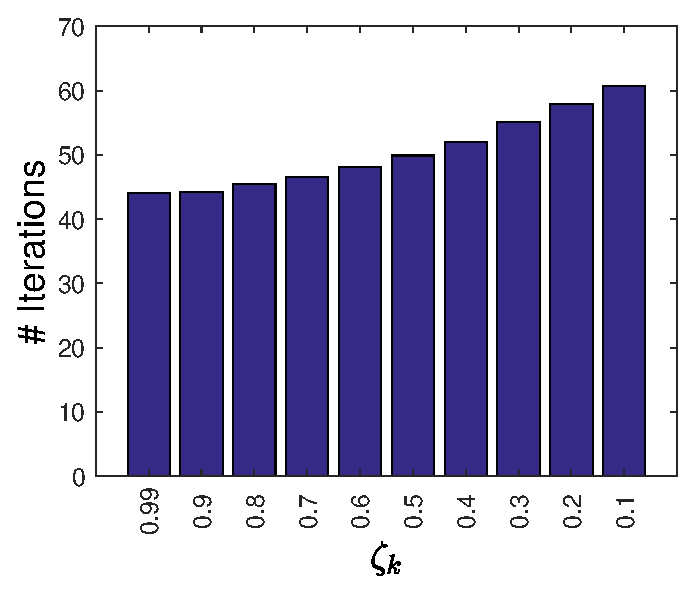
\includegraphics[scale=\myscaleF]{../figures/SDDit} & 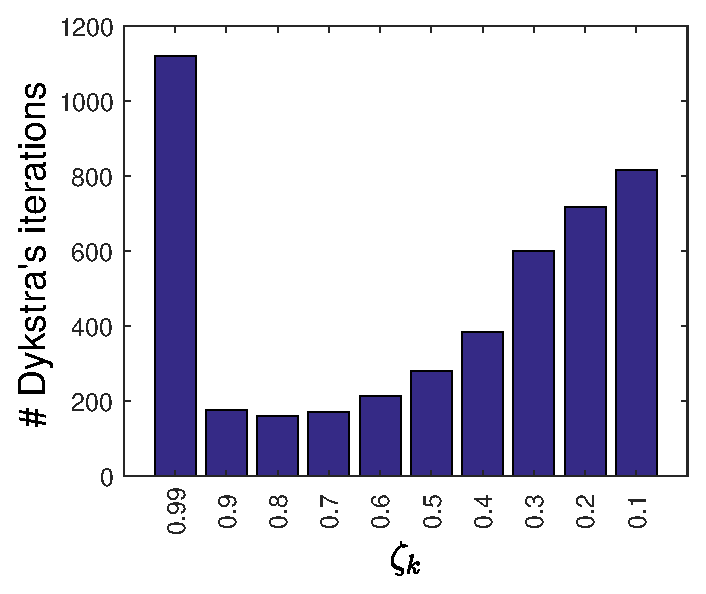
\includegraphics[scale=\myscaleF]{../figures/SDDDIT} & \includegraphics[scale=\myscaleF]{../figures/SDDtime} \\
			(a)                                                 & (b)                                                  & (c)                                                   \\
		\end{tabular}
		\caption{Results for 10 instances of Problem I using $n=100$, $m=200$, and $c=10$. Average number of: (a) iterations; (b) Dykstra’s iterations; (c)  CPU time in seconds needed to reach the solution for different choices of $\zeta_k$.}
	\end{figure}
\end{frame}

\begin{frame}[t]\frametitle{Influence of the inexact projection}
	\begin{figure}[H]\centering
		\begin{tabular}{ccc}
			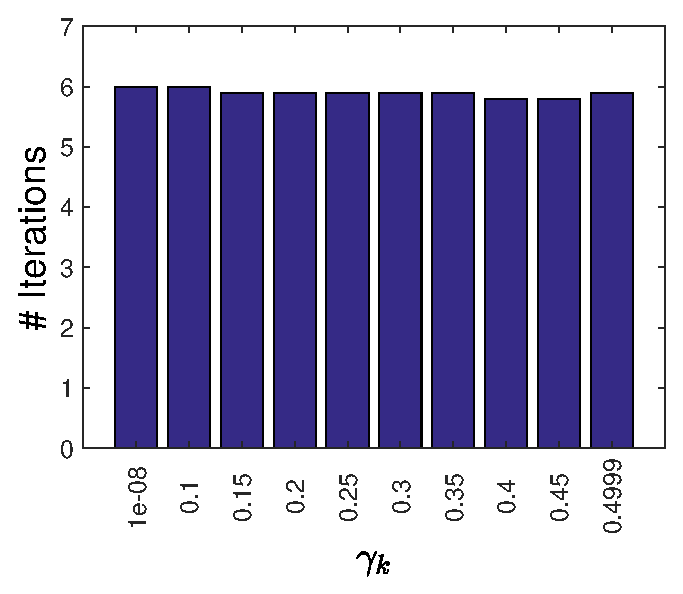
\includegraphics[scale=\myscaleF]{../figures/Specit} & 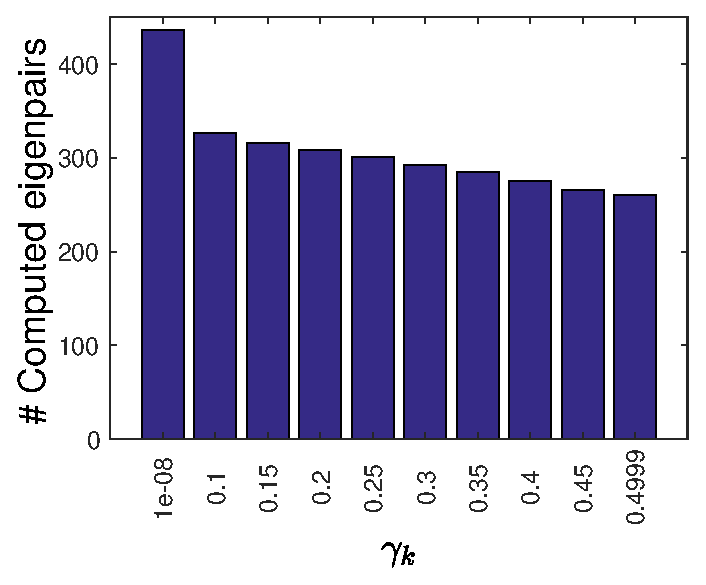
\includegraphics[scale=\myscaleF]{../figures/SpecFWIT} & \includegraphics[scale=\myscaleF]{../figures/Spectime} \\
			(a)                                                  & (b)                                                    & (c)                                                    \\
		\end{tabular}
		\caption{Results for 10 instances of Problem II using $n=800$, $m=1000$, and $c=100$. Average number of: (a) iterations; (b) computed eigenpairs; (c)  CPU time in seconds needed to reach the solution for different choices of $\gamma_k$.}
	\end{figure}
\end{frame}

\begin{frame}[t]\frametitle{Influence of the line search scheme}

	\begin{figure}[H]\centering
		\begin{tabular}{cccc}
			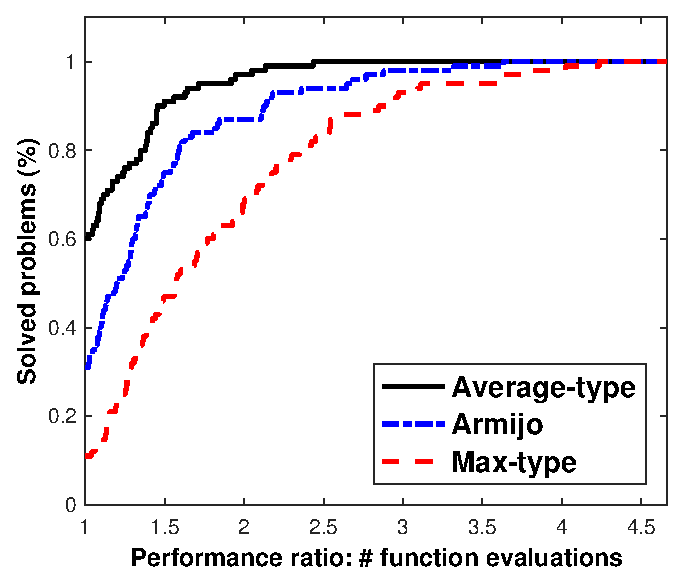
\includegraphics[scale=\myscale]{../figures/ppSDDnfev} & 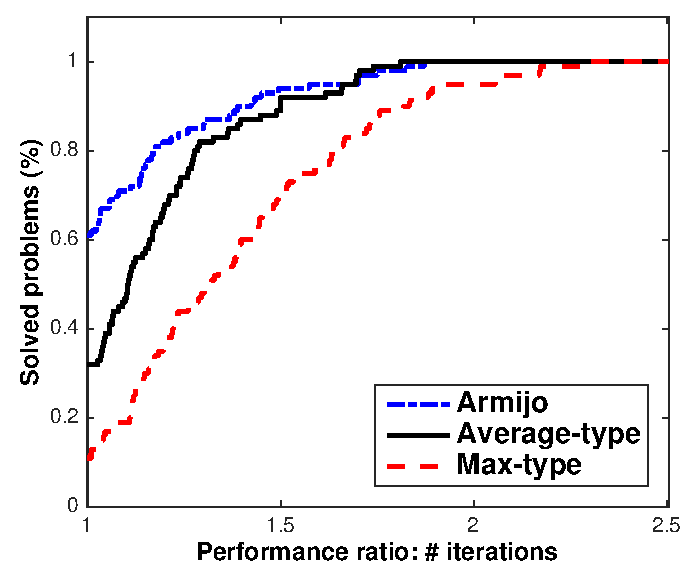
\includegraphics[scale=\myscale]{../figures/ppSDDit} & 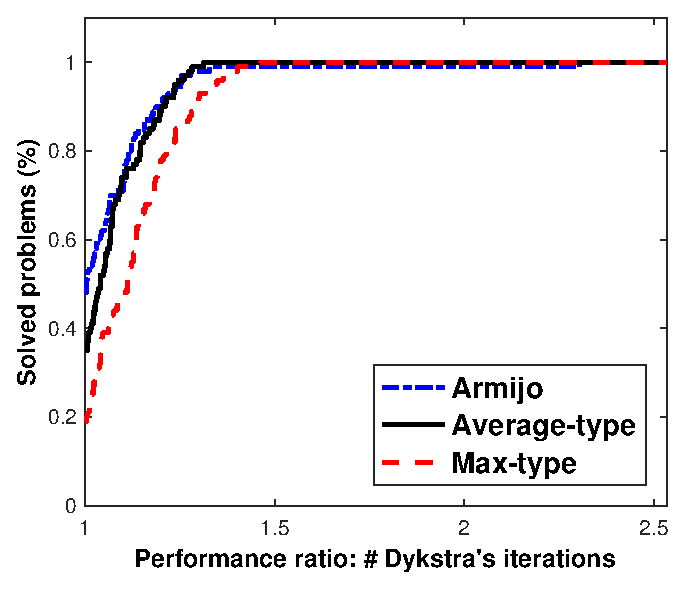
\includegraphics[scale=\myscale]{../figures/ppSDDnDIT} & 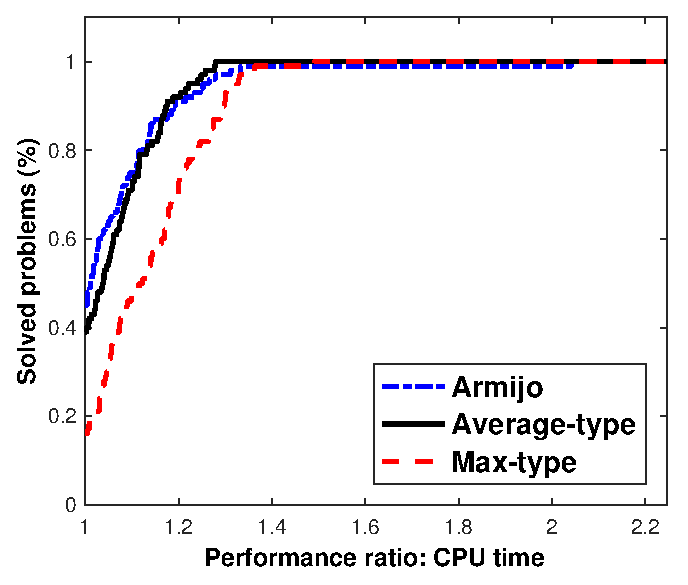
\includegraphics[scale=\myscale]{../figures/ppSDDtime} \\
			(a)                                                    & (b)                                                  & (c)                                                    & (d)                                                    \\
		\end{tabular}
		\caption{Performance profiles for Problem~I considering the SPG method with the Armijo, the Average-type, and the Max-type line searches strategies using as performance measurement: (a) number of function evaluations; (b) number of (outer) iterations; (c) number of Dykstra’s iterations; (d) CPU time.}

	\end{figure}
\end{frame}

\begin{frame}[t]\frametitle{Influence of the line search scheme}
	\begin{figure}[H]\centering
		\begin{tabular}{cccc}
			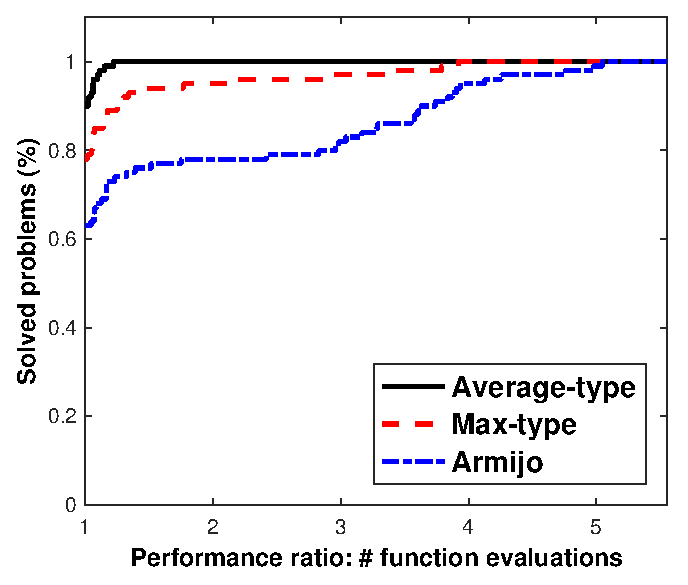
\includegraphics[scale=\myscale]{../figures/ppSpecnfev} & 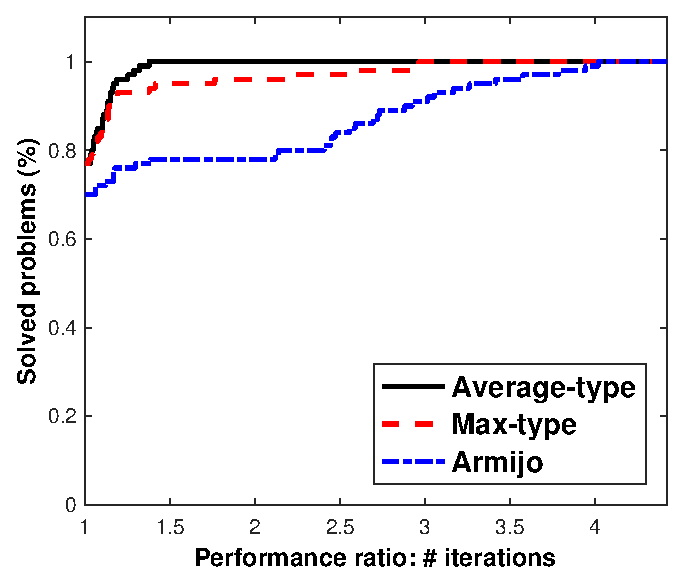
\includegraphics[scale=\myscale]{../figures/ppSpecit} & 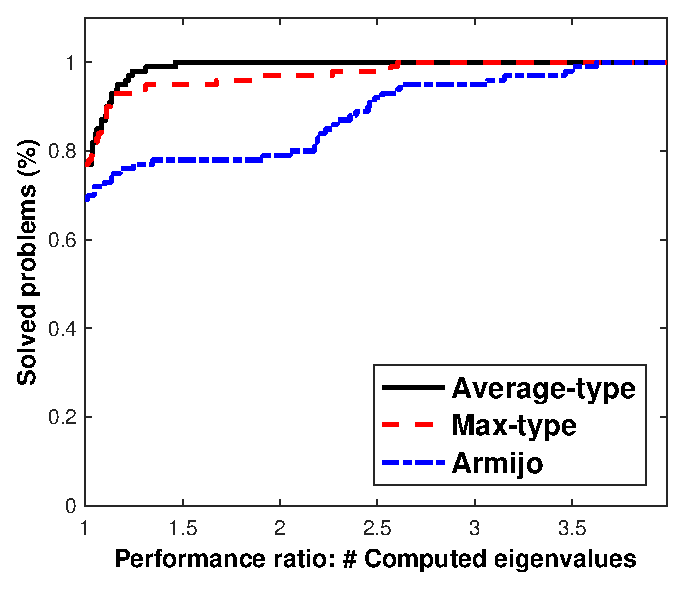
\includegraphics[scale=\myscale]{../figures/ppSpecnFW} & 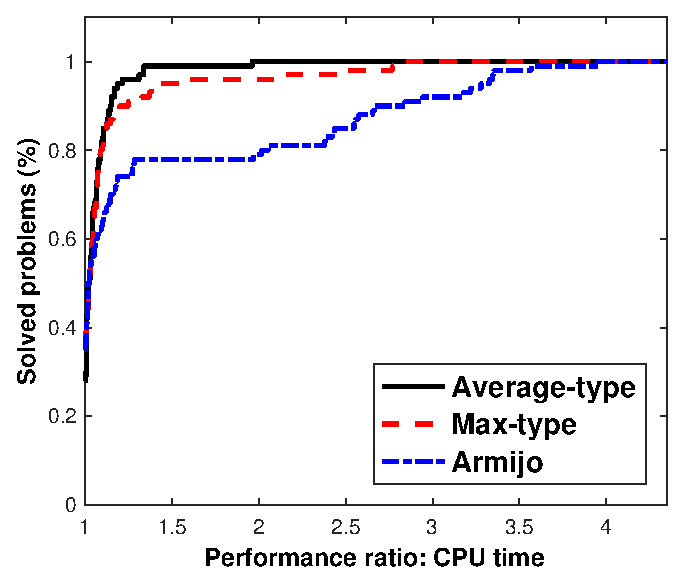
\includegraphics[scale=\myscale]{../figures/ppSpectime} \\
			(a)                                                     & (b)                                                   & (c)                                                    & (d)                                                     \\
		\end{tabular}
		\caption{Performance profiles for Problem~II considering the SPG method with the Armijo, the Average-type, and the Max-type line searches strategies using as performance measurement: (a) number of function evaluations; (b) number of (outer) iterations; (c) number of computed eigenpairs; (d) CPU time.}
	\end{figure}
\end{frame}
\chapter{Applications} \label{chap:App}

\section{Risks measures}

In this section we discuss different ways to measure the risk of portfolio.
\begin{definition}
	A portfolio with $n$ assets, $A_1, A_2, \dots, A_n$, is a vector $x^\top = (x_1, x_2, \dots, x_n)\in \R^n$ where each coordinate $x_i$ is the weight of capital invested in asset $A_i$.
\end{definition}
In finance risk is the possibility of a loss of capital and one way to measure risk is to calculate the probability of that loss happening.

Considering the loss as a random variable we can calculate the standard deviation of its distribution. This standard deviation (or \textit{volatility}) was considered a measure of risk by Nobel laureate in economics, Harry Markowitz in 1952 (see \cite{Markowitz1952}) under the hypothesis of loss has a normal distribution.

Others risk measures are done in terms of loss distribution percentiles. An upper percentile of the loss distribution is called \textit{Value-at-Risk} ($\mbox{VaR}_\beta$)\footnote{$\mbox{VaR}_\beta$ is the percentile of the loss distribution, i.e., with a specified confidence level $\beta$,  $\mbox{VaR}_\beta$ is the lowest amount $\zeta$ such that, with probability $\beta$, the loss is less or equal to $\zeta$.}. For instance, $\mbox{VaR}_{0.95}$ is an upper estimate of losses which is exceeded with 5\% probability. The popularity of $\mbox{VaR}_\beta$ is mostly related to a simple and easy to understand representation of high losses. $\mbox{VaR}_\beta$ can be quite efficiently estimated and managed when underlying risk factors are normally (log-normally) distributed.

An alternative measure of losses is another percentile risk measure which is called \textit{Conditional Value-at-Risk} ($\mbox{CVaR}_\beta$)\footnote{$\mbox{CVaR}_\beta$ is the average loss in the $100(1-\beta)$\% worst case scenarios.}. The $\mbox{CVaR}_\beta$ risk measure is closely related to $\mbox{VaR}_\beta$. For continuous distributions, $\mbox{CVaR}_\beta$ is defined as the conditional expected loss under the condition that it exceeds $\mbox{VaR}_\beta$, see Rockafellar and Uryasev (see \cite{RockafellarUryasev2001}). For continuous distributions, this risk measure also is known as \emph{Expected Shortfall}, \textit{Mean Excess Loss}, \textit{Mean Shortfall}, or \textit{Tail Value-at-Risk}.


\begin{figure}[H]
	\centering
	\includegraphics{figures/VarCvar.pdf}
	\caption{Portfolio Loss Distribution, VaR and CVaR.}
	\label{fig:VarCvar}
\end{figure}

\begin{remark}\normalfont\label{re:Normal}
If the loss distribution of a portfolio $x$ is normal, it follows that
\[
	\mu(x)+c\sigma(x)
\]
where $\mu(x)$ and $\sigma(x)$ denote the mean and volatility of the loss associated with portfolio $x$, and $c$ is a constant (see \cite[Chapter 2]{Roncalli2014}). If the portfolio manager has very optimistic forecasts, component $\mu(x)$ may substantially reduce the risk measure. This explains why omitting the mean component is standard practice in the asset management industry.
\end{remark}
% \begin{example}\normalfont
% 	We consider three stocks $A$, $B$ and $C$ whose current prices are respectively $\$ 15.00$, $\$ 25.00$ and $\$ 30.00$. We assume that their expected returns are equal to $30$ bps\footnote{1 bps or one basis point is equivalent to
% 		0.01\% (the hundredth part of 1\%) or 0.0001 in decimal form.}, $50$ bps and $20$ bps on a daily basis and their daily volatilities are $3\%$, $2\%$, and $1\%$ respectively. The asset correlation matrix is given by
% 	\[
% 		\rho = \left(
% 		\begin{array}{rrr}
% 				1.00 & 0.40 & 0.15 \\
% 				0.40 & 1.00 & 0.60 \\
% 				0.15 & 0.60 & 1.00
% 			\end{array}
% 		\right)
% 	\]

% 	We consider a portfolio composed by $100$ stocks $A$, $200$ stocks $B$ and $100$ stocks $C$. The value of this portfolio is $\$ 9,500.00$, being $\$ 1,500.00$ invested in stock $A$, $\$ 5,000.00$ in stock $B$ and $\$ 3,000.00$ in stock $C$, therefore the weights of the stocks in this portfolio are $15.79\%$, $52.63\%$, and $31.58\%$ respectively, so $x=(0.1579;\;0.5263;\; 0.3158)$. The expected loss of the portfolio is $\mu(x) = -30\times0.1579+50\times0.5263+20\times0.3158$, that is, $\mu(x) = -37$ bps. Using the relationship $\Sigma_{i,j}=\rho_{i,j}\sigma_1\sigma_j$ we find the covariance matrix
% 	\[
% 		\Sigma = \left(
% 		\begin{array}{llr}
% 				9.0 & 2.4 & 4.5 \\
% 				2.4 & 4.0 & 1.2 \\
% 				4.5 & 1.2 & 1.0
% 			\end{array}
% 		\right)\times10^{-4},
% 	\] since the volatility of portfolio is given by $\sigma^2(x) = x^\top \Sigma x$, we have that $\sigma(x) = 1.51\%$.

% 	Considering $\alpha = 0.99$, we have $\Phi^{-1}(0.99) = 2.325$ and
% 	$\phi(\Phi^{-1}(0.99))=\phi(2.325)=2.68\%$. Using the equations
% 	$(\ref{eq:var2})$ and $(\ref{eq:cvar2})$ we have

% 	\[
% 		\begin{aligned}
% 			\mathrm{VaR}_{99\%}(x) & = -0.37\% + 2.325 \times 1.51\% = 3.14\%              \\
% 			\mathrm{ES}_{99\%}(x)  & = -0.37\% + \frac{2.68}{0.01} \times 1.51\% = 3.68\%.
% 		\end{aligned}
% 	\]

% 	Risk can also be expressed in monetary terms, in this case,

% 	\[
% 		\begin{aligned}
% 			\mathrm{VaR}_{99\%}(x) & = 3.14\% \times \$ 9,500.00 = \$ 298.30  \\
% 			\mathrm{ES}_{99\%}(x)  & = 3.68\% \times \$ 9,500.00 = \$ 349.60.
% 		\end{aligned}
% 	\]
% 	According to the result of {\rm VaR}, in $99\%$ of the days, the loss will be less than $\$ 298.30$, however in the $1\%$ of the remaining days the {\rm VaR} does not measure how much great can be the loss, this is the role of {\rm CVaR} which indicates that the average loss will be $\$ 349.60$ on the worst $1\%$ days.
% \end{example}


\section{Portfolio optimization}

We consider a universe of $n$ assets. Let $x^\top = (x_1, x_2, \dots, x_n)$ be a portfolio and denoting by $R_i$ the return of asset $i$. If $R^\top=(R_1, R_2, \dots, R_n)$  is the random vector of asset returns then the return of portfolio $x$ is given by:
\[
	R(x) = x_1R_1+x_2R_2+\cdots x_nR_n = x^\top R.
\]
If we note $\mu$ and $\Sigma$ the vector of expected returns and the covariance matrix of asset returns, we deduce that the expected return of portfolio $x$ is equal to:
\[
	\mu(x) = x^\top \mu
\]
whereas its variance is given by:
\[
	\sigma^2(x) = x^\top \Sigma x.
\]
The mean-variance portfolio (MVP) of Markowitz (see \cite{Markowitz1952}) consists in maximizing the expected return $\mu(x)$ for a fixed value $\hat{\sigma}$ of the volatility $\sigma(x)$. This can be achieved by solving the problem:
\begin{eqnarray}\label{prob:MVP}
	\min_{x} \, \{- \mu(x)\}, \\
	\mbox{s.t. }\left\{
	\begin{aligned}\nonumber
		\sigma(x) = \hat{\sigma}, & \\
		\mathbf{1}^\top x=1       &
	\end{aligned}
	\right.
\end{eqnarray}
where $\textbf{1}^\top =(1,1,\dots,1)$, and the condition $\mathbf{1}^\top x=1$ means that the capital is fully invested.

A portfolio optimization  problem is defined when we want to minimize (or maximize) a performance measure subject to a set of constraints. Here are some examples of performance measures:

\begin{itemize}
	\item \textbf{Performance Measures}
	      \begin{itemize}
		      \item Expected return: $\mu(x)$;
		      \item Volatility: $\sigma(x)$;
		      \item Sharpe Ratio (SR): expected return per unit of risk
		            \[
			            \mbox{SR}(x) = \frac{x^\top \mu - r_f}{\sigma(x)}
		            \]
		            where $r_f$ is the risk-free rate (e.g. interest rate on a Treasury bill);
		      \item Information Ratio (IR): Sharpe Ratio with $r_f=0$;
		      \item $\mbox{VaR}_\beta$ (Value at Risk): quantile of the loss;
		      \item $\mbox{CVaR}_\beta$ (Conditional Value at Risk): expected value of the loss above some quantile.
	      \end{itemize}
\end{itemize}

Constraints can be:

\begin{itemize}
	\item \textbf{Constraints}
	      \begin{itemize}
		      \item Capital constraint: $\textbf{1}^\top x=1$;
		      \item Long-only constraint: $x\geq0$;
		      \item Self-financial constraint: $\textbf{1}^\top x=0$;
		      \item Holding constraint: $\mathbf{I}\leq x\leq \mathbf{J}$ where $\mathbf{I},\mathbf{J}\in\R^n$ are lower and upper bounds of the asset positions, respectively.
		      \item Leverage constraint: $\|x\|_1\leq K$.
	      \end{itemize}
\end{itemize}

Some known portfolio optimization problems are:

\noindent\textbf{Global Minimum Variance Portfolio (GMVP)}
\begin{eqnarray}\label{prob:GMVP}
	\min_{x} \,\{x^\top \Sigma x\}, \\
	\mbox{s.t. }\left\{
	\begin{aligned}\nonumber
		\mathbf{1}^\top x=1 \\
	\end{aligned}
	\right\}.
\end{eqnarray}

\noindent\textbf{Maximum Sharpe Ratio Portfolio (MSRP)}
\begin{eqnarray}\label{prob:MSRP}
	\max_{x} \,\{\mbox{SR}(x)\}, \\
	\mbox{s.t. }\left\{
	\begin{aligned}\nonumber
		\mathbf{1}^\top x=1 & \\
		\mathbf{0}\leq x \leq \mathbf{1}
	\end{aligned}
	\right.
\end{eqnarray}

We can also combine performances and constraints
\begin{eqnarray}\label{prob:General}
	\min_{x} \,\{\lambda \mbox{CVaR}_\beta(x) - \mu(x)\}, \\
	\mbox{s.t. }\left\{
	\begin{aligned}\nonumber
		\mathbf{1}^\top x=0 & \\
		\mathbf{0}\leq x \leq \mathbf{1}\\
		\|x\|_1\leq K.
	\end{aligned}
	\right.
\end{eqnarray}
where $\lambda$ is a parameter that controls how risk-averse the investor is.

All these problems aim to optimize a performance measure, we will present a new approach where the objective will be the risk allocation.

\section{Risk Parity}

Markowitz’s portfolio has never been fully embraced by practitioners, among other reasons because it only considers the risk of the portfolio as a whole and ignores the risk diversification (i.e., concentrates risk too much in few assets, this was observed in the 2008 financial crisis): one solution is the risk parity portfolio.

Risk parity is an approach to portfolio management that focuses on allocation of risk rather than allocation of capital. The risk parity approach asserts that when asset allocations are adjusted to the same risk level, the portfolio can achieve a higher Sharpe ratio and can be more resistant to market downturns.

While the minimum variance portfolio tries to minimize the variance (with the disadvantage that a few assets may be the ones contributing most to the risk), the risk parity portfolio distributes the weights so that the risk contribution of each asset (or asset class, such as bonds, stocks, real estate, etc.) is the same.

To define a risk-based allocation strategies it is necessary define how the risk of an asset affects the risk of the portfolio. 
Let $x^\top=(x_1,x_2,\dots,x_n)$ be a portfolio with $n$ assets and $\mathcal{R}(x)$ be a differentiable, homogeneous risk measure of $x$. Since $\mathcal{R}(x)$ is homogeneous, we have
\[
\mathcal{R}(x)=\frac{d}{d\lambda}\mathcal{R}(\lambda x)=\sum_{i=1}^n x_i \frac{\partial \mathcal{R} (x)}{\partial x_i}
\]
we can define the risk contribution of the asset $i$ by
$\mathcal{RC}_i$, where
\[
\mathcal{RC}_i(x)= x_i \frac{\partial \mathcal{R}(x)}{\partial x_i}.
\]
Therefore, the risk can be written as follows
\[
\mathcal{R}(x)=\sum_{i=1}^n \mathcal{RC}_i(x)
\]
which is known as \textbf{Euler's Allocation Principle}.

Volatility and $\mbox{CVaR}_\beta$  satisfy the properties required by the risk measure, $\mathcal{R}$, defined above. However, $\mbox{VaR}_\beta$ satisfies these properties only in the Gaussian case. When asset returns have a Normal Distribution, by simplicity (see Remark \ref{re:Normal}), we have that
$\mathcal{R}(x)=\sigma(x)=\sqrt{x^\top\Sigma x}$, it follows that
\[
\mathcal{RC}_i(x)= x_i \frac{\partial \sigma(x)}{\partial x_i}=\frac{x_i (\Sigma x)_i}{\sqrt{x^\top\Sigma x }}.
\]

It may be interesting for the investor to choose different risks for different assets, in this case the investor choose the percentage of risk that each asset should have in the portfolio, that is,
\begin{equation}\label{eq:RBP}
	\mathcal{RC}_i(x)=b_i\mathcal{R}(x),
\end{equation}
where $b_i$ represents the risk contribution that asset $i$ will have in the portfolio. Certainly $b_i\geq 0$ for all $i$ and
${\bf 1}^\top b =1$, with $b=(b_1, b_2, \dots, b_n)$. A portfolio distribution based in relation \eqref{eq:RBP} is called \textit{risk budgeting portfolio} (RBP), when $b_i=1/n$, for all $i$ the distribution is called \textit{risk parity portfolio} (RPP) or \textit{equal risk portfolio} (ERP).

In general, find the risk budgeting portfolio consists to solve the following non-linear system
\begin{eqnarray}\label{eq:SisNLin}
\mathcal{RC}_i(x)=b_i\mathcal{R}(x), \\
	\mbox{s.t. }\left\{
	\begin{aligned}\nonumber
b_i \geq 0, \\
x_i \geq 0, \\
{\bf 1}^\top b =1, \\
{\bf 1}^\top x =1.
	\end{aligned}
	\right.
\end{eqnarray}











Only in trivial cases can we find analytical solutions for this system, however, we can always find numerical solutions.

Consider $b^\top = (b_1, b_2, \dots, b_n)$, with ${\bf 1}^\top b =1$ and $f(x;b)$ defined by:
\[
f(x;b) = \sum_{i=1}^n \big(\mathcal{RC}_i(x) -b_i\mathcal{R}(x)\Big)^2
\] and the following optimization problem
\begin{eqnarray}\label{eq:MinProb}
\min_{x\geq \textbf{0}}\, \{f(x;b)\}; \\
	\mbox{s.t. }\left\{
	\begin{aligned}\nonumber
		\mathbf{1}^\top x=1 & \\
		\mathbf{0}\leq x \leq \mathbf{1}
	\end{aligned}
	\right.
\end{eqnarray}

If $x^\star$ is the solution to the problem (\ref{eq:MinProb}) and
$f(x^\star;b)=0$, so $x^\star$ is also system solution
(\ref{eq:SisNLin}). So we can use some optimization algorithm
quadratic to find a solution to the PDR. as it was
said before, to find a PPR just choose $b_i=1/n$, in the
process of choosing a PDR.

In the Gaussian case, when asset returns have a Normal distribution, we can consider $\mathcal{R}(x)=\sigma(x)$ and the system (\ref{eq:SisNLin}) reduces to
\begin{eqnarray}\label{eq:SisGauss}
x_i (\Sigma x )_i = b_i x^\top \Sigma x,\\
	\mbox{s.t. }\left\{
	\begin{aligned}\nonumber
b_i \geq 0, \\
x_i \geq 0, \\
{\bf 1}^\top b =1, \\
{\bf 1}^\top x =1.
	\end{aligned}
	\right.
\end{eqnarray}
for $i=1,2,\dots,n$.


Setting $w=x/\sqrt{x^\top \Sigma x}$, the equation $x_i (\Sigma x )_i = b_i x^\top \Sigma x$ is equivalent to $w_i(\Sigma w)_i =b_i$, or, in vector form
\[
\Sigma w = b/w.
\]

In 2013, Spinu (see in \cite{Spinu2013}) showed that the convex function
\[
f(w)= \frac{1}{2}w^\top \Sigma w - b^\top log(w)
\]
has a gradient equal to
\[
\nabla f(w) = \Sigma w - b/w
\]
and the system (\ref{eq:SisGauss}) can be reformulated by the following optimization problem
\begin{eqnarray}\label{eq:GaussProb}
\min_{x\geq {\bf 0}}\,\Big\{\frac{1}{2}w^\top \Sigma w - b^\top \log(w)\Big\};  \\
	\mbox{s.t. }\left\{
	\begin{aligned}\nonumber
		\mathbf{1}^\top x=1 & \\
		\mathbf{0}\leq x \leq \mathbf{1}
	\end{aligned}
	\right.
\end{eqnarray}


whose optimality condition is $\nabla f(w) = 0$ or $\Sigma w = b/w$ which is precisely the solution of the system (\ref{eq:SisGauss}).

















































\section{Case Study}




%           References      --------------------------------------
\topskip=2cm\advance\textheight by -2cm\enlargethispage{-1cm}

% \nocite{} % incluir sem citar no texto
% \nocite{*} % Citar todos

\printbibliography
%-----------------------------------------------------------------

\begin{frame}[c]\frametitle{}
	\centering
	\Huge \textbf{Thank you!}
\end{frame}
%-----------------------------------------------------------------
\end{document}
%-----------------------------------------------------------------